\documentclass{report}
\usepackage[utf8]{inputenc}
\usepackage[italian]{babel}
\usepackage[linktoc=all]{hyperref}
\usepackage{graphicx}
\usepackage{mathtools}
\usepackage{float}
\usepackage{wrapfig}
\usepackage{tabularx}

\graphicspath{ {./images/} }
\hypersetup{
	colorlinks,
	citecolor=black,
	filecolor=black,
	linkcolor=black,
	urlcolor=black
}
\usepackage[a4paper,includeheadfoot,margin=2.54cm]{geometry}
\usepackage{fancyhdr}
\newcommand\hr{\par\vspace{-.5\ht\strutbox}\noindent\hrulefill\par}
\usepackage{enumitem}
\newcommand{\code}{\texttt}

\begin{document}
	
	\begin{titlepage}
	\centering
	
\includegraphics[width=0.7\textwidth, keepaspectratio]{logounitn.jpg}

	\vspace{1.6cm}
	\LARGE{Dipartimento di Ingegneria e Scienza dell'Informazione\\}

	\vspace{1cm}
	\Large{Corso di Laurea in\\ Ingegneria dell'Informazione e Organizzazione d'Impresa}

	\vspace{1cm}
	\Huge\textsc{Appunti di Reti\\}
	\large{Dal materiale del prof. F. Granelli}

	\vspace{2cm}
	\Large{Autore}\\
	\large{Davide Parpinello}
	\\
	\vspace{2cm}
	\LARGE{Anno accademico 2019-2020}
	\end{titlepage}
	
	\tableofcontents
	\renewcommand{\chaptermark}[1]{%
		\markboth{#1}{}}
	\addtocontents{toc}{\protect\hypertarget{toc}{}}
	\pagestyle{fancy}
	\fancyhf{}
	\rhead{\hyperlink{toc}{Reti}}
	\lhead{\leftmark}
	\rfoot{\thepage}
	
	\chapter{Roadmap}
	\section{Internet}
	
	Internet è costituito da milioni di dispositivi, chiamati \textbf{sistemi terminali}, collegati tra loro da collegamenti in rame, fibre ottiche, oppure via radio come onde elettromagnetiche o satelliti.
	\medskip\\
	La frequenza di trasmissione in internet è data dall'ampiezza di banda disponibile.
	\medskip\\Sulla rete internet inoltre sono presenti particolari host, denominati \textbf{router}, che si occupano di instradare i pacchetti verso la loro destinazione finale.
	\medskip\\Nello scambio di messaggi tra host vengono implementati dei \textbf{protocolli}, che ne definiscono formato e ordine d'invio, così come le azioni intraprese in fase di trasmissione e/o ricezione di un messaggio o un altro evento.
	\medskip\\Internet è un'infrastruttura di comunicazione per applicazione distribuita, viene anche chiamato "rete delle reti" ed è organizzato in modo gerarchico.
	\section{Ai confini della rete}
	Sul bordo della rete internet troviamo applicazioni e sistemi terminali, raggruppati tra loro e connessi tra di loro mediante collegamenti cablati e wireless.
	\medskip\\I sistemi terminali (o host) fanno girare diversi programmi applicativi e possono essere organizzati con architettura client/server oppure P2P.
	\medskip\\L'accesso a internet può avvenire mediante diversi modi:
	\begin{itemize}
		\item \textbf{Accesso residenziale:} viene utilizzato un modem dial-up o DSL.
		\item \textbf{Accesso aziendale:} una LAN collega i sistemi terminali di aziende e università all'\textbf{edge router}, i sistemi terminali sono collegati tra loro mediante uno switch ethernet.
		\item \textbf{Accesso wireless:} i terminali vengono collegati mediante \textbf{access point}.
		\item \textbf{Reti domestiche:} sono costituite da un modem DSL o via cavo, un router/firewall/NAT, switch ethernet e accesso wireless. Spesso queste funzioni vengono raggruppate in un unico dispositivo (modem/router).
	\end{itemize}
	\section{Il nucleo della rete}
	Al centro della rete si trovano invece router interconnessi tra loro, che creano quindi una rete delle reti.
	\medskip\\I dati nel nucleo della rete vengono trasferiti con due modalità differenti:
	\begin{itemize}
		\item \textbf{Commutazione di circuito:} è presente un circuito dedicato per l'intera durata della sessione
		\item \textbf{Commutazione di pacchetto:} i messaggi di una sessione utilizzano le risorse su richiesta, di conseguenza potrebbero dover attendere per accedere a un collegamento.
	\end{itemize}
	\subsection{Esempio di commutazione di circuito}
	Consideriamo un file L di 640.000 bit, un bitrate totale C da 1.536 Mbps, TDM con 24 slot/s, 500ms per stabilire la connessione.
	\medskip\\ Trovo inizialmente la capacità di un singolo slot:\[C_{1 slot} = \frac{C}{24} = 0.064 Mbps = 64 Kbps\]
	Successivamente calcolo il tempo necessario alla trasmissione:\[T_{tx} = \frac{L}{C_{1 slot}} = 10s\]
	Infine, calcolo il tempo totale:\[T_{tot}=500ms+10s=10,5s\]
	\subsection{Esempio di commutazione di circuito}
	I secondi necessari per trasmettere un pacchetto in uscita su un collegamento da R bps sono dati da L/R, mentre il ritardo 3L/R
	\subsection{Confronto fra commutazione di pacchetto e di circuito}
	La commutazione di pacchetto consente un utilizzo della rete da parte di maggiori utenti, ed è ottima per i dati a raffica.\medskip\\ Dal lato negativo, presenta un'eccessiva congestione, causando ritardi e perdite di pacchetti. Sono quindi necessari protocolli per il trasferimento affidabile e per il controllo della congestione.
	\subsection{Struttura gerarchica}
	La rete internet ha una struttura fondamentalmente gerarchica:
	\begin{itemize}
		\item Al centro sono presenti \textbf{ISP di livello 1}, che offrono una copertura nazionale e/o internazionale
		\begin{itemize}
			\item Comunicano tra loro come fossero pari
		\end{itemize}
		\item \textbf{ISP di livello 2:} ISP più piccoli, copertura nazionale/distrettuale.
		\begin{itemize}
			\item Si può connettere solo ad alcuni ISP di livello 1 e ad altri di livello 2
			\item Paga l'ISP di livello 1 che gli fornisce la connettività per il resto della rete
		\end{itemize}
		\item \textbf{ISP di livello 3 e ISP locali (di accesso):}
		\begin{itemize} 
			\item sono le reti "ultimo salto", le più vicine agli host
			\item Sono clienti degli ISP di livello superiore che li collegano all'intera internet.
		\end{itemize}
	\end{itemize}
	Un pacchetto attraversa un sacco di reti, dal livello più basso fino al principale e poi nuovamente a scendere.
	\section{Ritardi, perdite e throughput nelle reti a comunicazione di pacchetto}
	Nella rete si verificano dei ritardi quando il tasso di arrivo dei pacchetti eccede la capacità di evaderli, con la conseguenza che vengono accodati nei buffer del router in attesa del proprio turno. Se non ci sono buffer liberi i pacchetti vengono scartati e ritrasmetti dal nodo precedente o, in alcuni casi, non venire proprio ritrasmessi.
	\medskip\\ Quattro cause di ritardo dei pacchetti sono le seguenti:
	\begin{enumerate}
		\item Ritardo di elaborazione sul nodo
		\begin{itemize}
			\item Controllo errori sui bit
			\item Determinazione del canale di uscita
		\end{itemize}
		\item Ritardo di accodamento
		\begin{itemize}
			\item Attesa di trasmissione
			\item Livello di congestione del router
		\end{itemize}
		\item Ritardo di trasmissione (L/R)
		\begin{itemize}
			\item R = frequenza di trasmissione del collegamento
			\item L = lunghezza del pacchetto
		\end{itemize}
		\item Ritardo di propagazione (d/s)
		\begin{itemize}
			\item d = lunghezza dl collegamento fisico 
			\item s = velocità di propagazione del collegamento (\textasciitilde \(2 \cdot 10^8\) m/s)
		\end{itemize}
	\end{enumerate}
	\begin{center}
		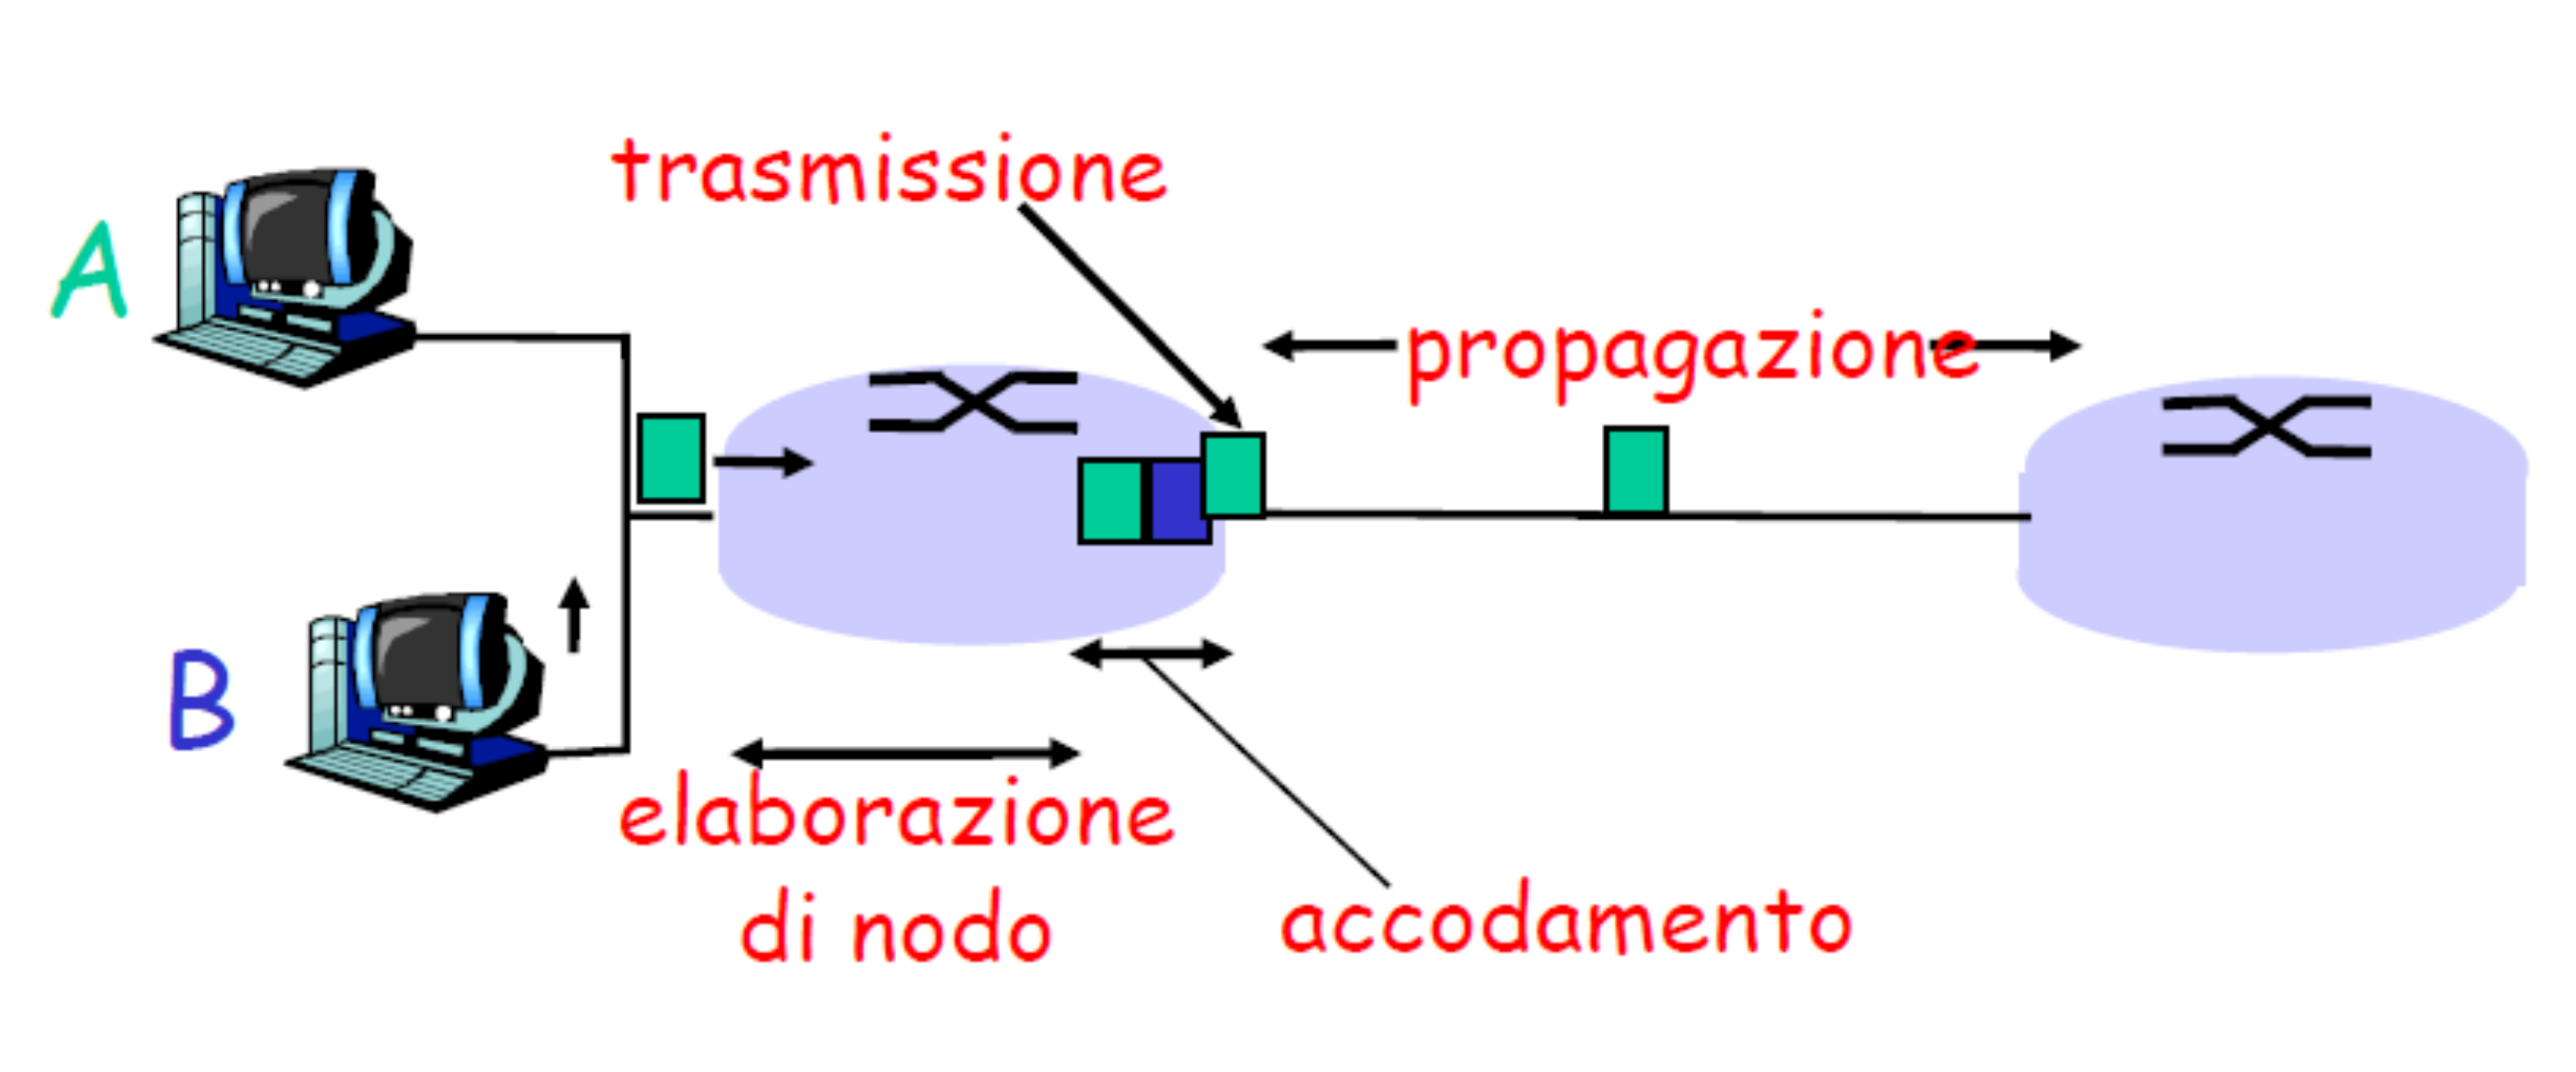
\includegraphics[width=0.7\linewidth]{ritardi.png}
	\end{center}
	\subsection{Ritardo di un nodo}
	Il ritardo di un nodo è dato dalla seguente formula:
	\begin{equation}
		d_{nodal} = d_{proc}+d_{queue}+d_{trans}+d_{prop}
	\end{equation}
	dove:
	\begin{itemize}
		\item d\textsubscript{proc} = ritardo di elaborazione (processing delay)
		\subitem- in genere di pochi microsecondi, o anche meno
		\item d\textsubscript{queue} = ritardo di accodamento
		\subitem- dipende dalla congestione
		\item d\textsubscript{trans} = ritardo di trasmissione (transmission delay)
		\subitem- significativo sui collegamenti a bassa velocità
		\item d\textsubscript{prop} = ritardo di propagazione (propagation delay)
		\subitem- da pochi microsecondi a centinaia di millisecondi
	\end{itemize}
	\subsubsection{Ritardo di accodamento}
	\begin{itemize}
		\item R = frequenza di trasmissione (bps)
		\item L = lunghezza del pacchetto (bit)
		\item a = tasso medio di arrivo dei pacchetti
	\end{itemize}
	
	Se calcoliamo La/R otteniamo l'intensità di traffico:
	\begin{itemize}
		\item Vicino a 0: poco ritardo
		\item Minore o uguale a 1: traffico consistente
		\item Maggiore di 1: più lavoro in arrivo di quanto possa essere effettivamente svolto, ritardo medio infinito.
	\end{itemize}
	Il \textbf{throughput} viene calcolato come la frequenza (bit/unità di tempo) alla quale i bit sono trasferiti tra mittente e ricevente. Può essere istantaneo o medio (in un periodo più lungo).
	\medskip\\In internet si considera anche il \textbf{collo di bottiglia}, ovvero un collegamento su un percorso punto-punto che vincola un throughput end to end.
	\section{Livelli di protocollo e i loro modelli di servizio}
	Si considerano principalmente 5 livelli di protocollo:
	\begin{enumerate}
		\item \textbf{Applicazione:} di supporto alle applicazioni di rete
		\item \textbf{Trasporto:} trasferimento dei messaggi del livello applicazione tra modulo client e server, connessione tra processi applicativi
		\item \textbf{Rete:} instradamento dei datagram dall'origine al destinatario
		\item \textbf{Link \textit{(collegamento)}:} instradamento dei datagram attraverso una serie di commutatori di pacchetto
		\item \textbf{Fisico:} trasferimento dei singoli bit
	\end{enumerate}
	\section{Reti sotto attacco: la sicurezza}
	I malintenzionati installano malware negli host attraverso internet. Il malware può raggiungere gli host attraverso virus, worm o cavalli di Troia. Un malware di spionaggio può registrare quanto viene digitato, i siti visitati e informazioni di upload. Gli host infettati possono diventare botnet e essere usati per lo spamming e attacchi DDoS. Un malware è spesso auto-replicante e da un host attaccato può passare ad altri host.
	\paragraph{Analisi di pacchetti} Chiamato anche packet sniffing, quando un'interfaccia di rete legge/registra tutti i pacchetti che la attraversano.
	\paragraph{IP spoofing} Invio di pacchetti con un indirizzo sorgente falso.
	\paragraph{Record-and-playback} Vengono "sniffati" dati sensibili per utilizzarli in un secondo momento.
	\chapter{Il livello Applicazione}
	\section{Principi delle applicazioni di rete}
	Le applicazioni di rete sono costruite con diverse architetture
	\begin{itemize}
		\item Client-Server
		\begin{itemize}
			\item L'host (o client) interagisce direttamente con il server
			\item Più client ci sono più il servizio diminuisce
		\end{itemize}
		\item Peer-to-Peer (P2P)
		\begin{itemize}
			\item Non c'è un server sempre attivo
			\item Coppie arbitrarie di host comunicano direttamente fra di loro
			\item Facilmente scalabile ma difficile da gestire
		\end{itemize}
		\item Architetture ibride
		\begin{itemize}
			\item Skype, messaggistica istantanea
			\item Connessione client-client, utilizzo del server per la ricerca dell'indirizzo della parte remota
		\end{itemize}
		\item Cloud computing
		\begin{itemize}
			\item Un insieme di tecnologie che permettono sia di archiviare dati che elaborarli tramite l'utilizzo di risorse distribuite e virtualizzate in rete
			\item Creazione di copie di sicurezza preventive in modo automatico trasferendo tutta l'operatività online
			\item Dati memorizzati in server farm
			\item Sempre client-server ma basata sulla virtualizzazione
		\end{itemize}
	\end{itemize}
	Un processo è un programma in esecuzione su un host. All'interno dell'host due processi comunicano utilizzando schemi di interprocesso, mentre su host differenti comunicano attraverso lo scambio di messaggi.
	\begin{itemize}
		\item \textbf{Processo client:} processo che dà inizio alla comunicazione
		\item \textbf{Processo server:} processo che attende di essere contattato
	\end{itemize}
	Un processo invia/riceve messaggi mediante la sua socket. La socket è analoga ad una porta mediante la quale un processo che vuole inviare un messaggio lo fa uscire. Questo presuppone l’esistenza di un’infrastruttura esterna che trasporterà il messaggio attraverso la rete fino alla porta del processo di destinazione.
	\medskip\\ Per il trasporto internet vengono utilizzati i servizi dei protocolli TCP e UDP.
	\subsubsection{Servizio TCP}
	\begin{itemize}
		\item \textcolor{red}{Orientato alla connessione:} è richiesto un setup fra i processi client e server
		\item \textcolor{red}{Trasporto affidabile} fra i processi d'invio e ricezione
		\item \textcolor{red}{Controllo di flusso:} il mittente non vuole sovraccaricare il destinatario
		\item \textcolor{red}{Controllo della congestione:} "strozza" il processo d'invio quando la rete è sovraccaricata
		\item \textbf{Non offre} temporizzazione, garanzie sull'ampiezza di banda minima, sicurezza
		\item \textbf{Più affidabile ma si paga con ritardi di trasferimento}
	\end{itemize}
	\subsubsection{Servizio UDP}
	\begin{itemize}
		\item Trasferimento dati inaffidabile fra processi d'invio e ricezione
		\item \textbf{Non offre} setup della connessione, affidabilità, controllo di flusso, controllo della congestione, temporizzazione né ampiezza di banda minima e sicurezza
		\item \textcolor{red}{Mandare i dati il più velocemente possibile ma senza completa affidabilità}, usato per gaming online e VoIP
	\end{itemize}
	\section{Web e HTTP}
	L'HTTP, o HyperText Transfer Protocol, è un protocollo a livello applicazione per il web, che considera un client che richiede, riceve e visualizza gli oggetti del Web e un server, che invia gli oggetti in risposta ad una richiesta.
	\medskip\\Viene utilizzato TCP nel seguente modo:
	\begin{itemize}
		\item Il client inizializza la connessione TCP con il server (crea una socket) tipicamente sulla porta 80
		\item Il server accetta la connessione TCP dal client
		\item Avviene lo scambio di messaggi HTTP tra browser e server web
		\item Chiusura della connessione TCP
	\end{itemize}
	HTTP è un protocollo \textit{stateless} (senza stato), cioè il server non mantiene informazioni sulle richieste fatte dal client.
	\medskip\\Le connessioni HTTP possono essere non persistenti o persistenti.
	\paragraph{RTT} Round trip time, tempo impiegato da un piccolo pacchetto per andare dal client al server e ritornare al client.
	\subsection{Connessioni non persistenti}
	Viene trasferito un solo oggetto su una singola connessione TCP. Il tempo di risposta è dato da:
	\begin{itemize}
		\item Un RTT per inizializzare la connessione TCP
		\item Un RTT per inviare la richiesta HTTP e i primi byte
		\item Il tempo necessario alla trasmissione del file
	\end{itemize}
	Quindi totale = 2 RTT + tempo di trasmissione. Le connessioni non persistenti presentano alcuni svantaggi:
	\begin{itemize}
		\item Richiedono 2RTT per ogni oggetto
		\item Overhead dell'OS per ogni connessione TCP
		\item I browser aprono spesso connessioni TCP parallele per caricare gli oggetti referenziati
	\end{itemize}
	\subsection{Connessioni persistenti}
	Il server lascia la connessione TCP aperta dopo l'invio di una risposta, i successivi messaggi tra gli stessi client/server vengono trasmessi sulla connessione aperta, il client invia le richieste non appena incontra un oggetto referenziato, un solo RTT per tutti gli oggetti referenziati.
	\subsection{Messaggi HTTP}
	I messaggi HTTP possono essere di richiesta o di risposta.
	\subsubsection{Richiesta HTTP}
	\begin{verbatim}
		GET /somedir/page.html HTTP/1.1
		Host: www.someschool.edu
		User-agent: Mozilla/4.0
		Connection: close Accept-language:fr
	\end{verbatim}
	\subsubsection{Tipi di metodi}
	La versione HTTP/1.0 fornisce i seguenti metodi per effettuare le richiese:
	\begin{itemize}
		\item \textbf{GET:} richiesta solamente mediante URL
		\item \textbf{POST:} vengono inseriti nel corpo della richiesta anche dati da inviare al server
		\item \textbf{HEAD:} chiede al server di escludere l'oggetto richiesto dalla risposta
	\end{itemize}
	Nella versione HTTP/1.1 vengono aggiunti i seguenti metodi:
	\begin{itemize}
		\item \textbf{PUT:} include il file nel corpo dell'entità e lo invia al percorso specificato nel campo URL
		\item \textbf{DELETE:} cancella il file specificato nel campo URL
	\end{itemize}
	\subsubsection{Risposta HTTP}
	\begin{verbatim}
		HTTP/1.1 200 OK
		Connection close
		Date: Thu, 06 Aug 1998 12:00:15 GMT
		Server: Apache/1.3.0 (Unix)
		Last-Modified: Mon, 22 Jun 1998 ...
		Content-Length: 6821
		Content-Type: text/html
	\end{verbatim}
	\subsubsection{Codici di stato della risposta HTTP}
	Nella prima riga del messaggio di risposta sono inclusi codice di stato e relativa espressione in base all'esito della richiesta. Alcuni codici sono i seguenti:
	\begin{itemize}
		\item \textbf{200 OK:} La richiesta ha avuto successo, oggetto inviato nella risposta
		\item \textbf{301 Moved Permanently:} Oggetto trasferito nella nuova posizione indicata da \verb|Location|
		\item \textbf{400 Bad Request:} il messaggio di richiesta non è stato compreso dal server
		\item \textbf{404 Not Found:} il documento richiesto non si trova su questo server
		\item \textbf{505 HTTP Version Not Supported:} il server non ha la versione di protocollo HTTP indicata
	\end{itemize}
	\subsection{Cookies}
	\begin{center}
		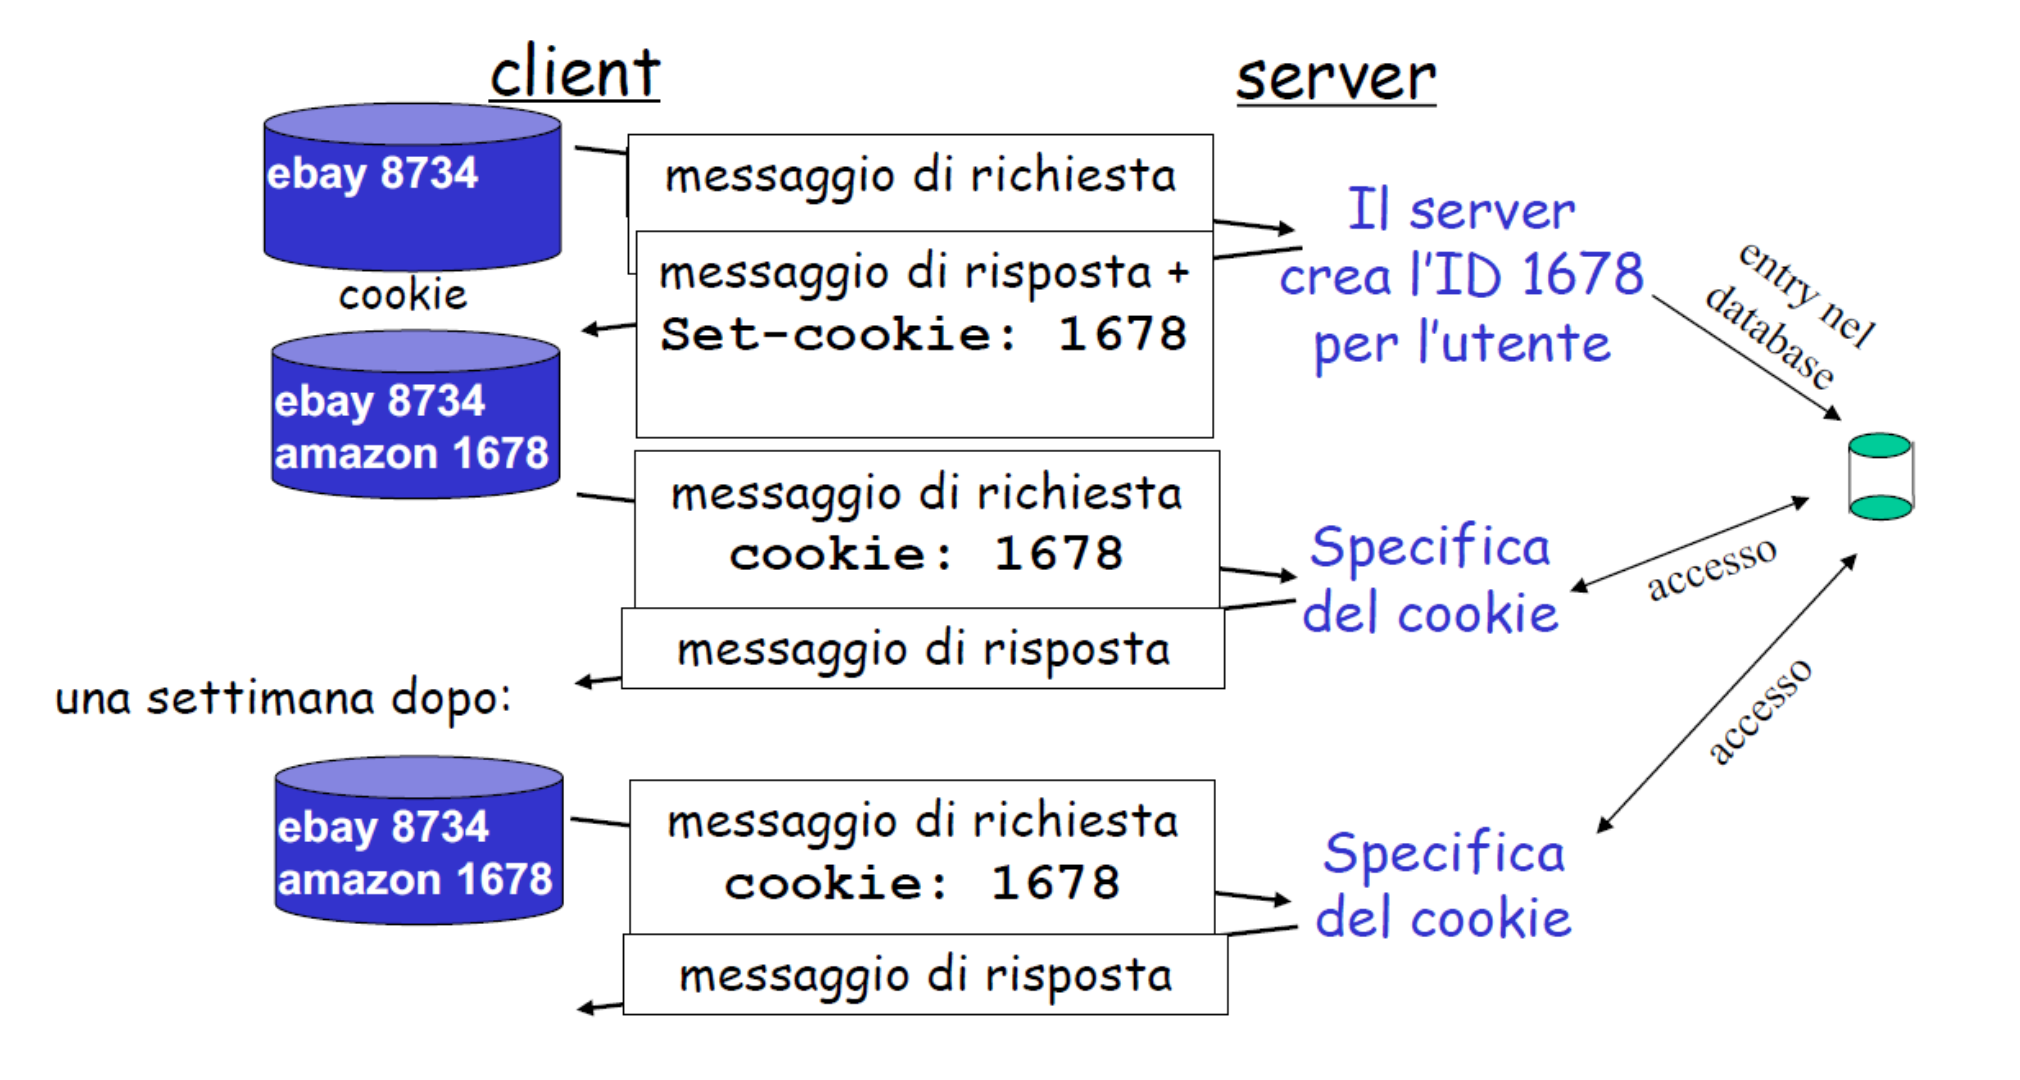
\includegraphics[width=0.7\linewidth]{cookies.png}
	\end{center}
	I cookies possono essere utilizzati per: autorizzazioni, dati carte per acquisti, raccomandazioni all'utente e possono mantenere lo stato del mittente e del ricevente per più transazioni; i messaggi HTTP trasportano lo stato. I cookies permettono ai siti di imparare molte cose sugli utenti.
	\subsection{Cache web (server proxy)}
	L'obiettivo di una web cache è quello di soddisfare la richiesta del client senza coinvolgere il server d'origine. La cache opera come client e come server, e consente di ridurre i tempi di risposta alle richieste dei client, riducendo il traffico sul collegamento a internet.
	\paragraph{GET condizionale} Ha l'obiettivo di non inviare un oggetto se la cache ne ha una copia aggiornata. 
	\\Per questo la cache specifica la data della copia dell'oggetto nella richiesta HTTP: \verb|If-modified-since: <date>|
	\\A lato server la risposta non contiene l'oggetto se la copia nella cache è aggiornata: \verb|HTTP/1.0 304 not modified|
	\subsection{HTTP/2.0}
	È un’evoluzione di HTTP, che mantiene quindi i metodi HTTP, i codici di stato e la semantica migliorando però le prestazioni.
	\section{FTP}
	FTP, o File Transfer Protocol, viene utilizzato per trasferire file con un host remoto. Il server FTP opera solitamente sulla porta 21. Vengono aperte due connessioni, prima una di controllo e successivamente, se andata a buon fine la prima, una seconda per il trasferimento del file. La connessione di controllo è quindi "fuori banda" (out of band). Il server FTP mantiene lo stato
	\subsection{Comandi comuni}
	\begin{itemize}
		\item \verb|USER username|
		\item \verb|PASS password|
		\item \verb|LIST| elenca i file della directory corrente
		\item \verb|RETR filename| recupera un file dalla directory corrente
		\item \verb|STOR filename| memorizza un file nell'host remoto
	\end{itemize}
	\subsection{Codici di ritorno comuni}
	\begin{itemize}
		\item \verb|331 Username OK, password required|
		\item \verb|125 data connection already open; transfer starting|
		\item \verb|425 Can't open data connection|
		\item \verb|452 Error writing file|
	\end{itemize}
	\section{Posta elettronica}
	La posta elettronica è costituita da tre componenti principali: agente utente, server di posta, SMTP (Simple Mail Transfer Protocol).
	\paragraph{Agente utente} Detto anche mail reader, si occupa della composizione, editing e lettura dei messaggi di posta elettronica (esempi: Outlook, Thunderbird). I messaggi in uscita sono memorizzati sul server.
	\paragraph{Server di posta} In esso è contenuta la casella di posta (mailbox) che contiene i messaggi in arrivo per l'utente e la coda dei messaggi da trasmettere.
	\paragraph{Protocollo SMTP} Utilizzato tra i server per inviare messaggi: il client è il server di posta trasmittente e il server il ricevente. Viene utilizzato TCP per trasferire in modo affidabile i messaggi di posta dal client al server sulla porta 25; il trasferimento è diretto. Ci sono tre fasi per il trasferimento: handshaking (saluto), trasferimento dei messaggi e chiusura. L'SMTP utilizza connessioni persistenti.
	\medskip\\Esistono poi diversi protocolli di accesso alla posta:
	\begin{itemize}
		\item POP: Post Office Protocol. Utilizzato per autorizzazione e download
		\item IMAP: Internet Mail Access Protocol. Ha più funzioni e consente di manipolare i messaggi memorizzati sul server.
		\item HTTP: GMail, Hotmail, ecc...
	\end{itemize}
	\paragraph{POP3} Suddiviso in due fasi: autorizzazione e transazione, è un protocollo senza stato tra le varie sessioni
	\paragraph{IMAP} Mantiene tutti i messaggi sul server, consente all'utente di organizzare i messaggi in cartelle e conserva lo stato tra le varie sessioni (nomi delle cartelle, associazione tra identificatori dei messaggi e nomi delle cartelle).
	\section{DNS}
	Il DNS, Domain Name System è un protocollo a livello applicazione che consente a host, router e server DNS di comunicare per risolvere i nomi dei siti web. Il DNS traduce un hostname come \textit{www.facebook.com} in un indirizzo IP.
	\paragraph{Host aliasing} In alcuni casi, un host può avere più nomi, come nel caso dell'aliasing dei server mail.
	\medskip\\Il DNS è un database distribuito implementato in una gerarchia di server DNS. Tipicamente, un server DNS radice viene contattato da un server DNS locale che non può tradurre un nome. A sua volta, il DNS radice contatta un server DNS autorizzato se non conosce la mappatura del nome, la ottiene e la restituisce al server DNS locale.
	\paragraph{Server TLD (top-level domain} Si occupano dei domini .com, .org, .net, .edu, ecc. e di tutti gli altri domini locali di alto livello, quali .uk, .fr, .ca e .jp.
	\paragraph{Server di competenza (authoritative server} Ogni organizzazione dotata di host internet pubblicamente accessibili (server web e di posta) deve fornire i record DNS di pubblico dominio che mappano i nomi di tali host in indirizzi IP; possono essere mantenuti dall'organizzazione o dal service provider.
	\medskip\\Il server DNS locale non appartiene strettamente alla gerarchia dei server, ciascun ISP (università, società) ha un server DNS locale. Quando un host effettua una richiesta DNS, la query viene inviata al suo server DNS locale, che opera da proxy e inoltra la query in una gerarchia di server DNS.
	\medskip\\Le query DNS possono essere effettuate in due modalità: iterativa o ricorsiva. Nel caso di query iterativa, il server contattato risponde con il nome del server da contattare, nel caso in cui non riesca a risolvere il nome; sarà quindi compito dell'host iniziale contattare quel server. Nel caso di query ricorsiva l'host affida il compito di tradurre il nome al server DNS contattato; in questo caso sarà il server stesso a contattare un secondo server per risolvere il nome, al quale può a sua volta assegnare il compito in modo iterativo.
	\medskip\\Una volta che un server DNS impara la mappatura la mette nella cache, dove le informazioni vengono invalidate dopo un certo periodo di tempo. Tipicamente, un server DNS locale memorizza nella cache gli indirizzi IP dei server TLD, quindi i server radice non vengono visitati spesso.
	\medskip\\Il DNS è un database distribuito che memorizza i record di risorsa (RR) che hanno il seguente formato: \verb|(name, value, type, TTL)|
	\begin{itemize}
		\item Type = A
		\begin{itemize}
			\item \code{name} è il nome dell'host (server)
			\item \code{value} è l'indirizzo IP
		\end{itemize}
		\item Type = NS
		\begin{itemize}
			\item \code{name} è il dominio (\code{foo.com})
			\item \code{value} è il nome dell'host del server DNS di competenza di questo dominio
		\end{itemize}
		\item Type = CNAME
		\begin{itemize}
			\item \code{name} è il nome alias di qualche nome canonico (\code{www.ibm.com})
			\item \code{value} è il nome canonico (\code{servereast.backup2.ibm.com})
		\end{itemize}
		\item Type = MX
		\begin{itemize}
			\item \code{value} è il nome del server di posta associato a \code{name}
		\end{itemize}
	\end{itemize}
	\subsection{Protocollo DNS}
	Il protocollo DNS è costituito da domande (query) e messaggi di risposta, entrambi con lo stesso formato.
	\subsubsection{Intestazione del messaggio (12 byte - 6 campi)}
	L'intestazione è costituita da un numero da 16 bit di identificazione della domanda, utilizzato uguale dalla risposta, e da un flag indicante:
	\begin{itemize}
		\item domanda o risposta
		\item richiesta di ricorsione
		\item ricorsione disponibile
		\item risposta di competenza
	\end{itemize}
	\subsubsection{Resto del messaggio}
	\begin{itemize}
		\item Campi per il nome richiesto e il tipo di domanda
		\item RR nella risposta alla domanda
		\item Record per i server di competenza
		\item Informazioni extra che possono essere usate
	\end{itemize}
	\newpage
	\section{Condivisione di file P2P}
	Nell'architettura P2P pura non c'è un server sempre attivo, infatti coppie arbitrarie di host (peer) comunicano direttamente tra loro. I peer non devono essere sempre attivi e possono cambiare indirizzo IP.
	\subsection{Confronto tra architettura server client e P2P}
	\begin{center}
		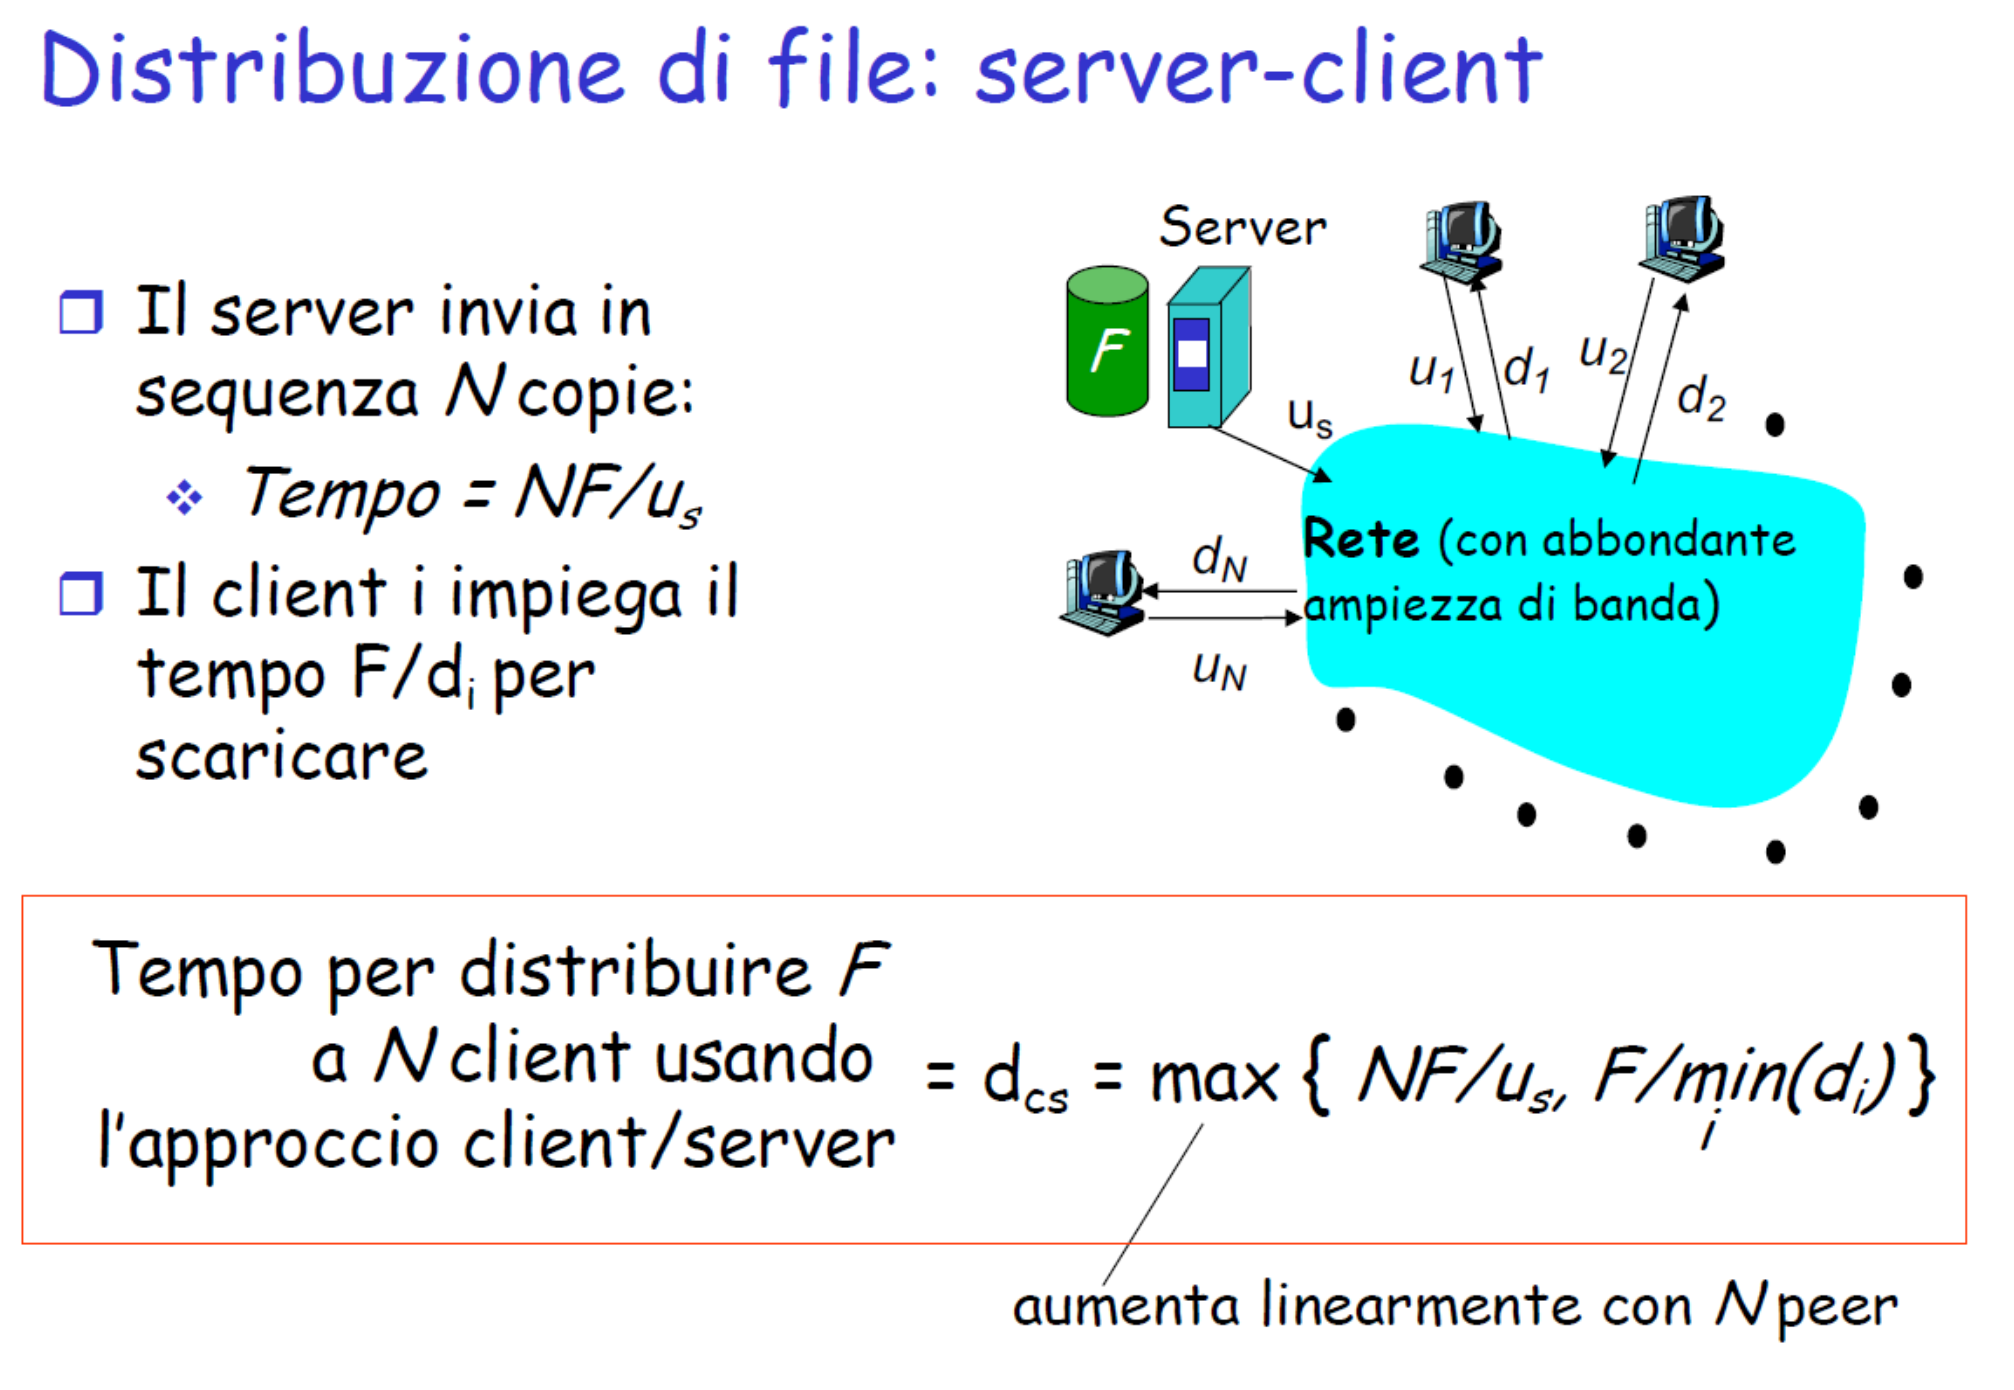
\includegraphics[width=0.7\linewidth]{server-client.png}
		\medskip\\
		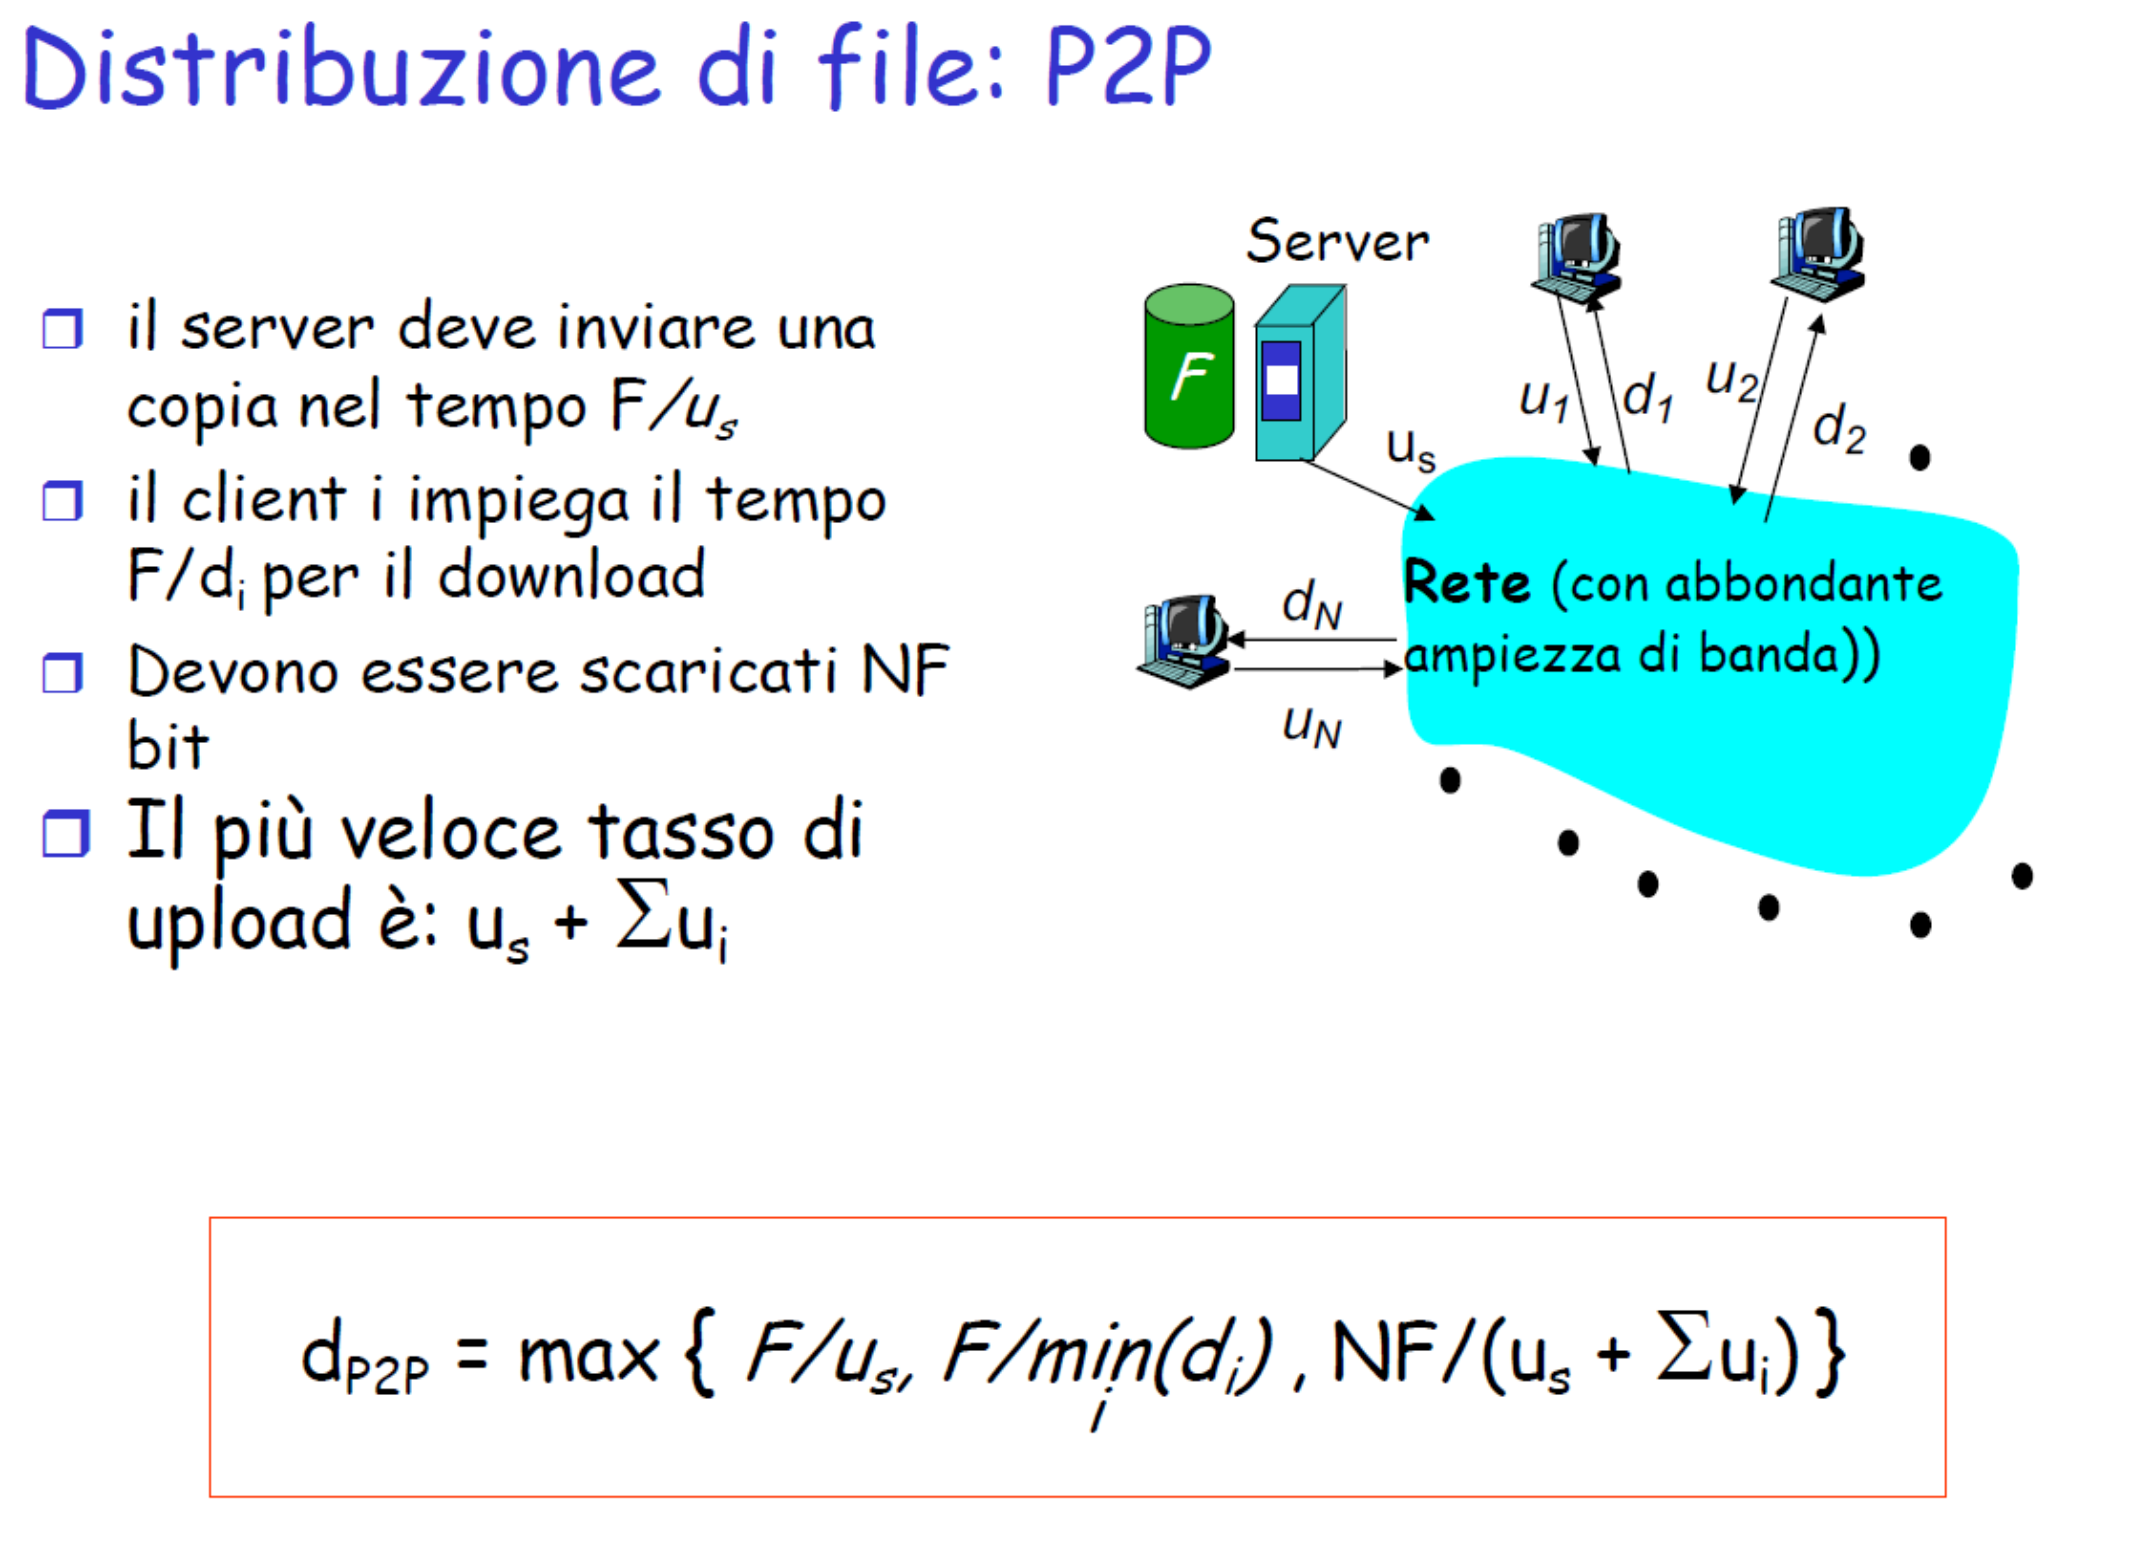
\includegraphics[width=0.7\linewidth]{p2p.png}
	\end{center}
	\paragraph{Tracker} Il tracker tiene traccia dei peer che partecipano alla rete, dove un torrent è un gruppo di peer che si cambiano parti di un file.
	\medskip\\Un file condiviso è diviso in più parti da 256 Kb, chiamati \textit{chunk}. Il peer invia le sue parti a 4 vicini, quelli che gli stanno inviando alla frequenza più alta (aggiornata ogni 10 secondi). Successivamente, ogni 30 secondi viene scelto un peer a caso che riceve i chunk; oltre a questi 5 gli altri peer non riceveranno nulla.
	\paragraph{Query flooding} Ciascun peer indicizza i file che rende disponibili per la condivisione. Il messaggio di richiesta è trasmesso sulle connessioni TCP esistenti, il peer inoltra la richiesta e il messaggio di successo più trasmesso viene inviato sul percorso inverso.
	\section{Cloud Computing}
	L'architettura del cloud computing prevede uno o più server reali, generalmente in architettura ad alta affidabilità e fisicamente collocati presso i datacenter del fornitore del servizio.
	\subsection{CDN}
	Le CDN, o Content Delivery Networks, rappresentano una soluzione comune per la realizzazione di servizi su internet, la quale costruisce una rete "overlay" per la distribuzione di contenuti. Serve per memorizzare i dati il più vicino possibile ai consumatori in modo da ottimizzare le prestazioni di rete, ridurre la latenza ed evitare colli di bottiglia.
	\chapter{Il livello di Trasporto}
	\section{Servizi a livello di trasporto}
	I servizi a livello di trasporto forniscono la comunicazione logica tra processi applicativi di host differenti. I protocolli di trasporto vengono eseguiti nei sistemi terminali: il lato invio scinde i messaggi in segmenti e li passa al livello di rete, il lato ricezione invece riassembla i segmenti in messaggi e li passa al livello applicazione.
	\begin{itemize}
		\item \textbf{Livello di rete:} si occupa della comunicazione logica tra host
		\item \textbf{Livello di trasporto:} si occupa della comunicazione logica tra processi, si basa sui servizi del livello di rete e li potenzia
	\end{itemize}
	\paragraph{Demultiplexing} Nell'host ricevente, si occupa di consegnare i segmenti ricevuti alla socket appropriata.
	\paragraph{Multiplexing} Nell'host mittente, raccoglie i dati da varie socket, li incapsula con l'intestazione (usata poi nel demultiplexing).
	\newline
	\begin{wrapfigure}{r}{0.3\textwidth}
		\centering
		\vspace{-20pt}
		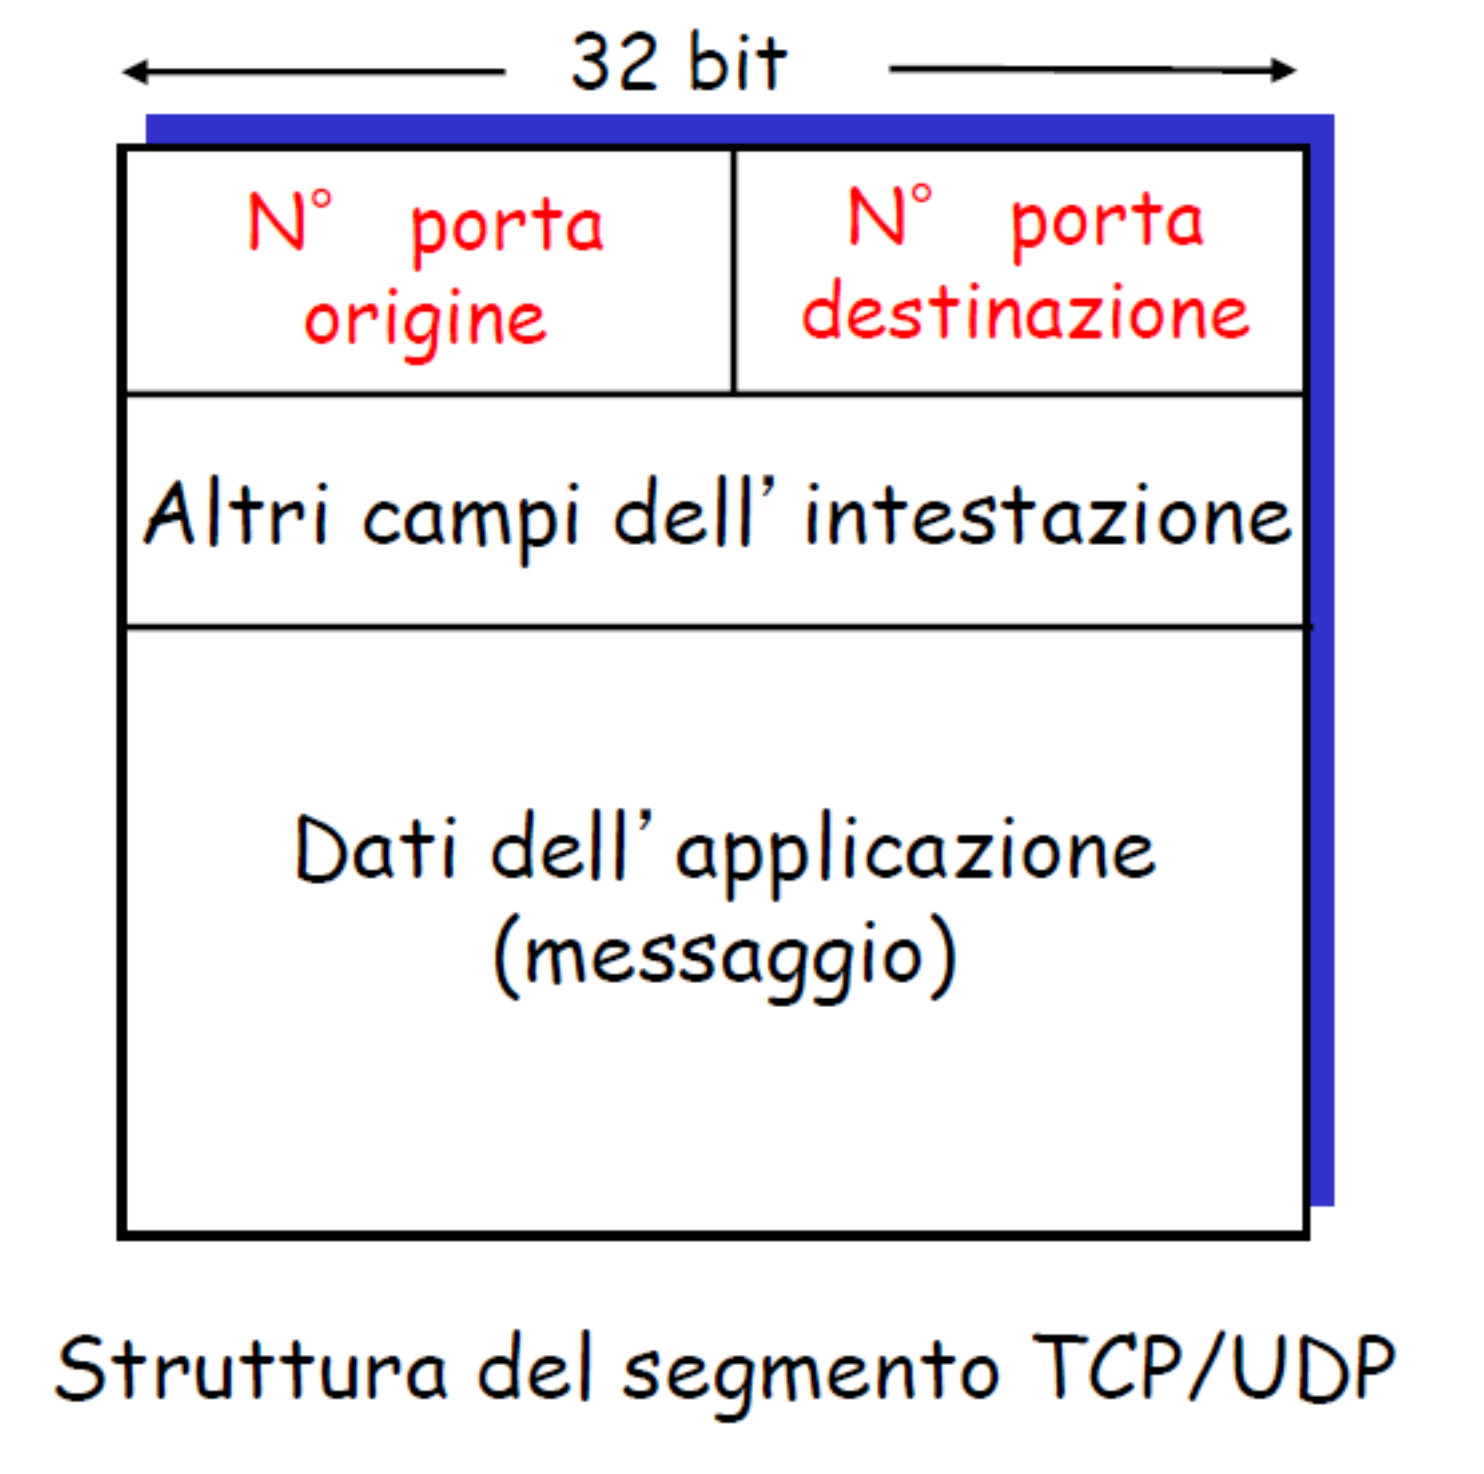
\includegraphics[width=0.25\textwidth]{segmento-trasporto}
		\vspace{-30pt}
	\end{wrapfigure}
	L’host riceve i datagrammi IP; ogni datagramma ha un indirizzo IP di origine e uno di destinazione, e trasporta 1 segmento a livello di trasporto, ogni segmento ha un numero di porta di origine e un numero di porta di destinazione. L’host usa gli indirizzi IP e i numeri di porta per inviare il segmento alla socket appropriata.
	
	\subsection{Demultiplexing senza connessione}
	Il demultiplexing senza connessione utilizza una socket UDP identificata da indirizzo IP di destinazione e numero della porta di destinazione. Quando l'host riceve il segmento UDP controlla il numero di porta nel segmento e poi lo invia alla socket correlata. Datagram IP con indirizzi IP e/o numeri di porta di origine differenti vengono inviati alla stessa socket.
	\begin{center}
		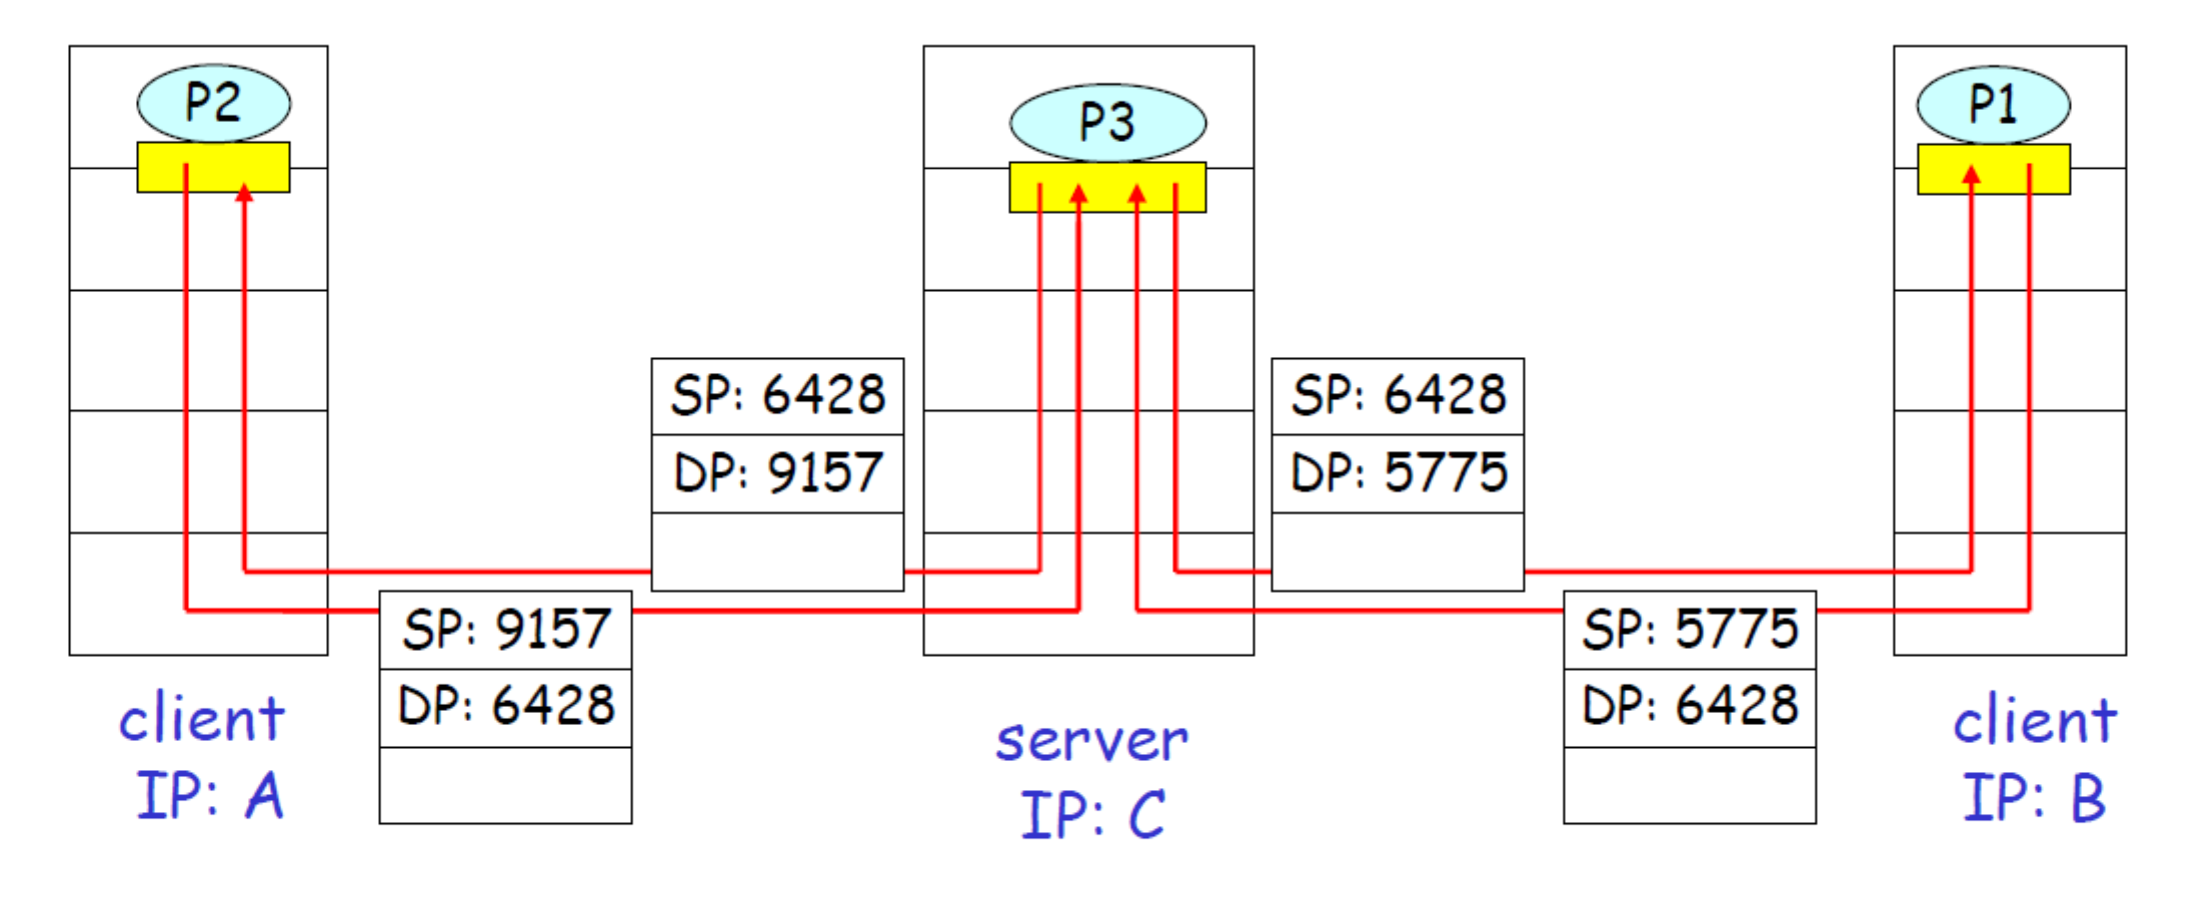
\includegraphics[width=0.7\linewidth]{socket-udp}
		\text{Demultiplexing senza connessione}
	\end{center}
	\subsection{Demultiplexing orientato alla connessione}
	Il demultiplexing orientato alla connessione utilizza una socket TCP identificata da quattro parametri: indirizzo IP e porta d'origine e indirizzo IP e porta di destinazione. L'host ricevente usa tutti e quattro i parametri per inviare il segmento alla socket appropriata. Un host server può supportare più socket TCP contemporanee. I server web hanno socket differenti per ogni connessione client, con HTTP non-persistente si avrà invece una socket differente per ogni richiesta.
	\begin{center}
		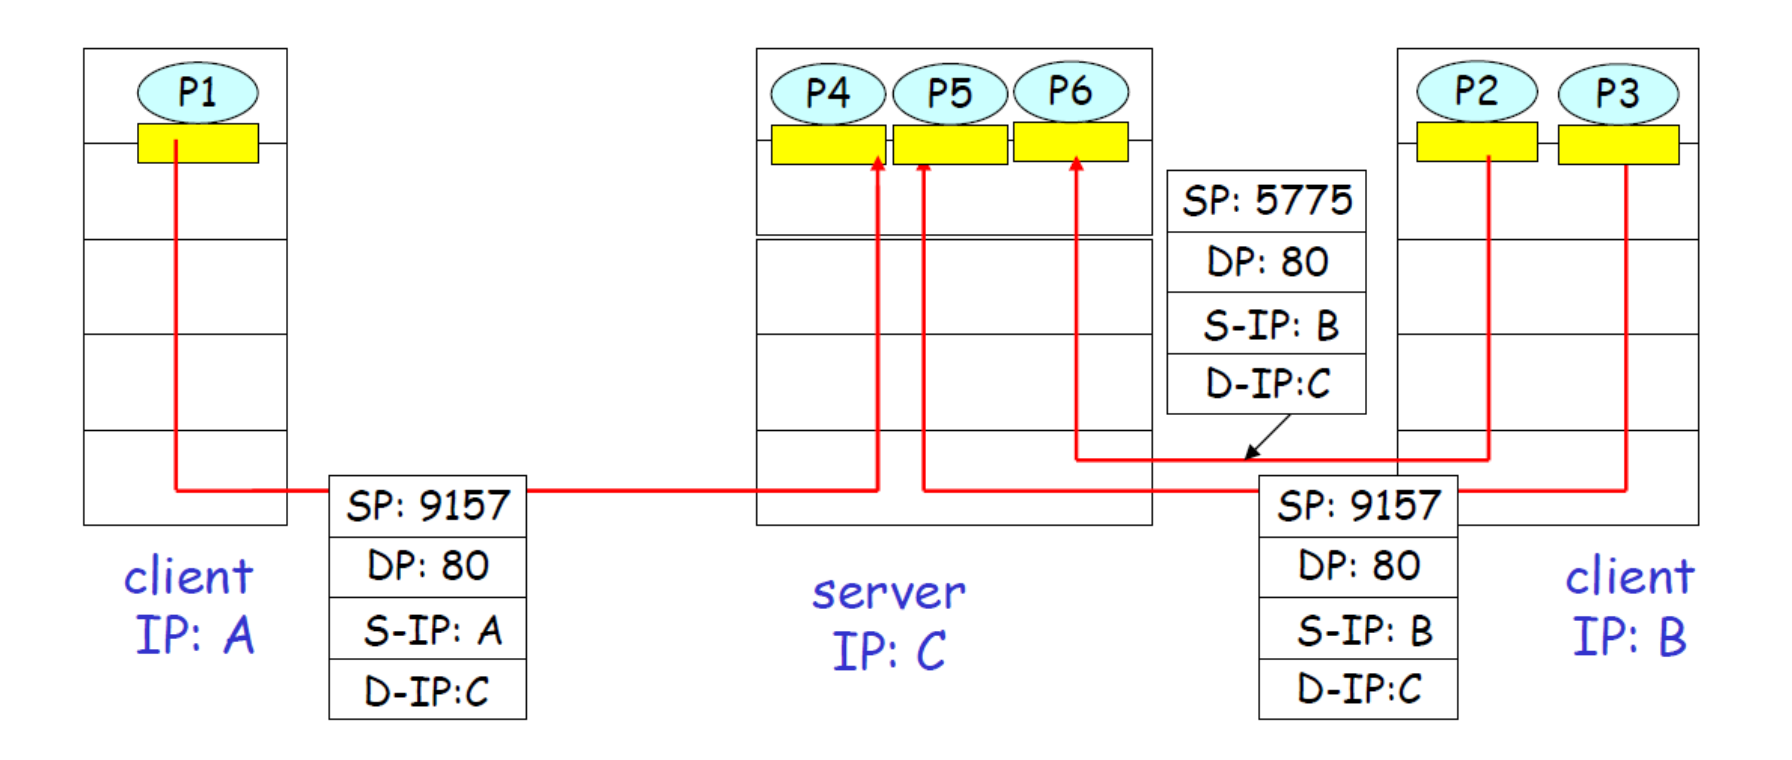
\includegraphics[width=0.7\linewidth]{socket-tcp}
	\end{center}
	\section{Trasporto senza connessione: UDP}
	\begin{wrapfigure}{r}{0.3\textwidth}
		\centering
		\vspace{-30pt}
		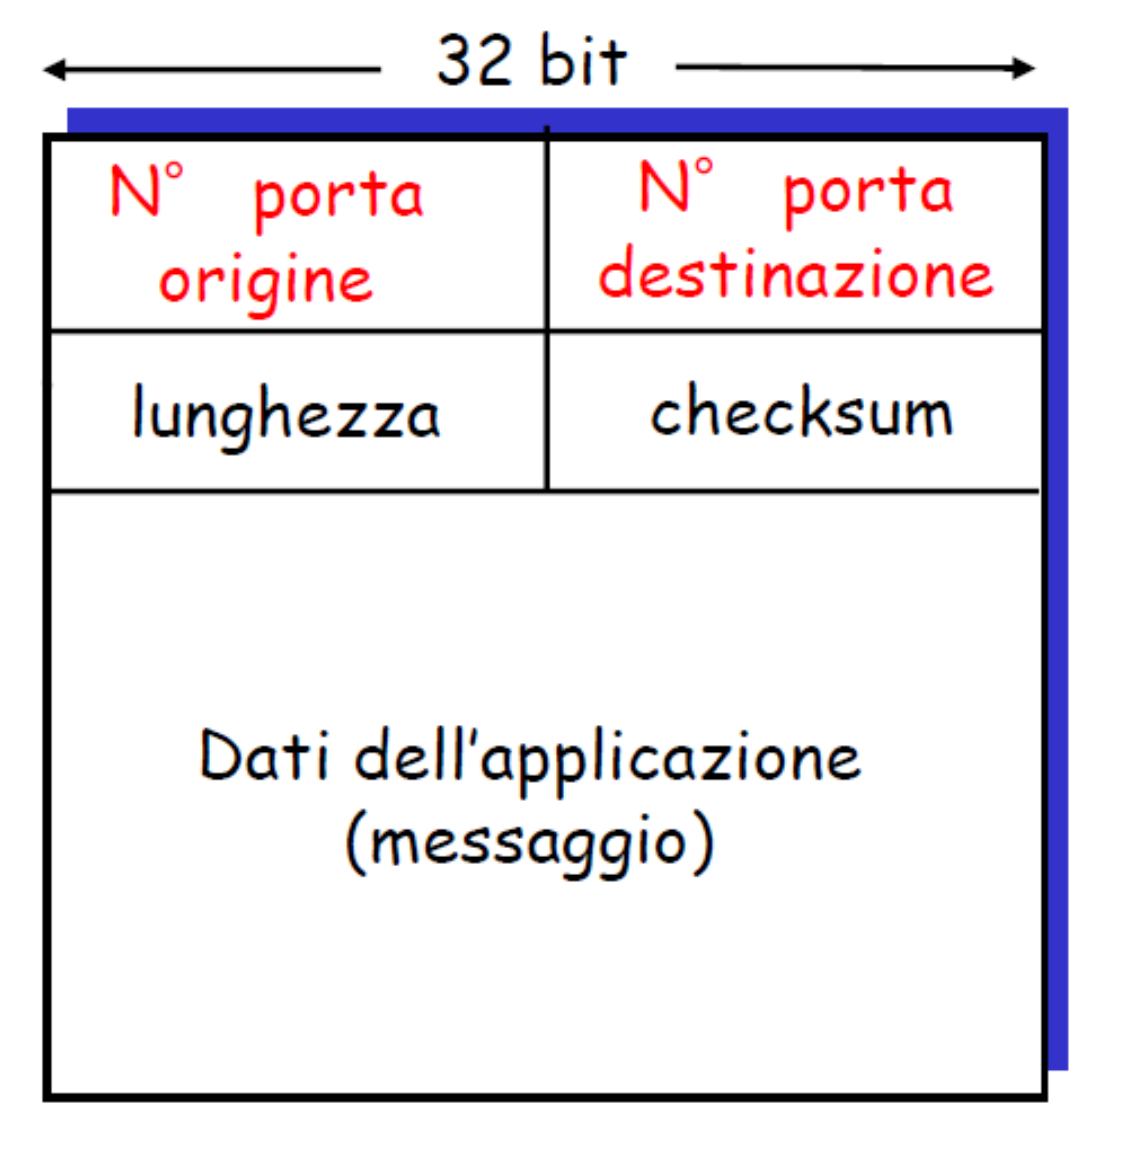
\includegraphics[width=0.25\textwidth]{segmento-udp}
		\vspace{-20pt}
	\end{wrapfigure}

	UDP, User Datagram Protocol, è un protocollo di trasporto "senza fronzoli", infatti ha un servizio di consegna best effort (miglior sforzo). Per questo i segmenti UDP possono essere perduti o consegnati fuori sequenza all'applicazione.\medskip\\ Essendo senza connessione non c'è handshaking tra mittente e destinatario, quindi ogni segmento UDP è gestito indipendentemente dagli altri.
	\paragraph{Checksum UDP} Il checksum UDP serve per rilevare gli “errori” (bit alternati) nel segmento trasmesso, il segmento viene trattato come una sequenza di interi da 16 bit.

	\section{Principi del trasferimento dati affidabile}
	\begin{center}
		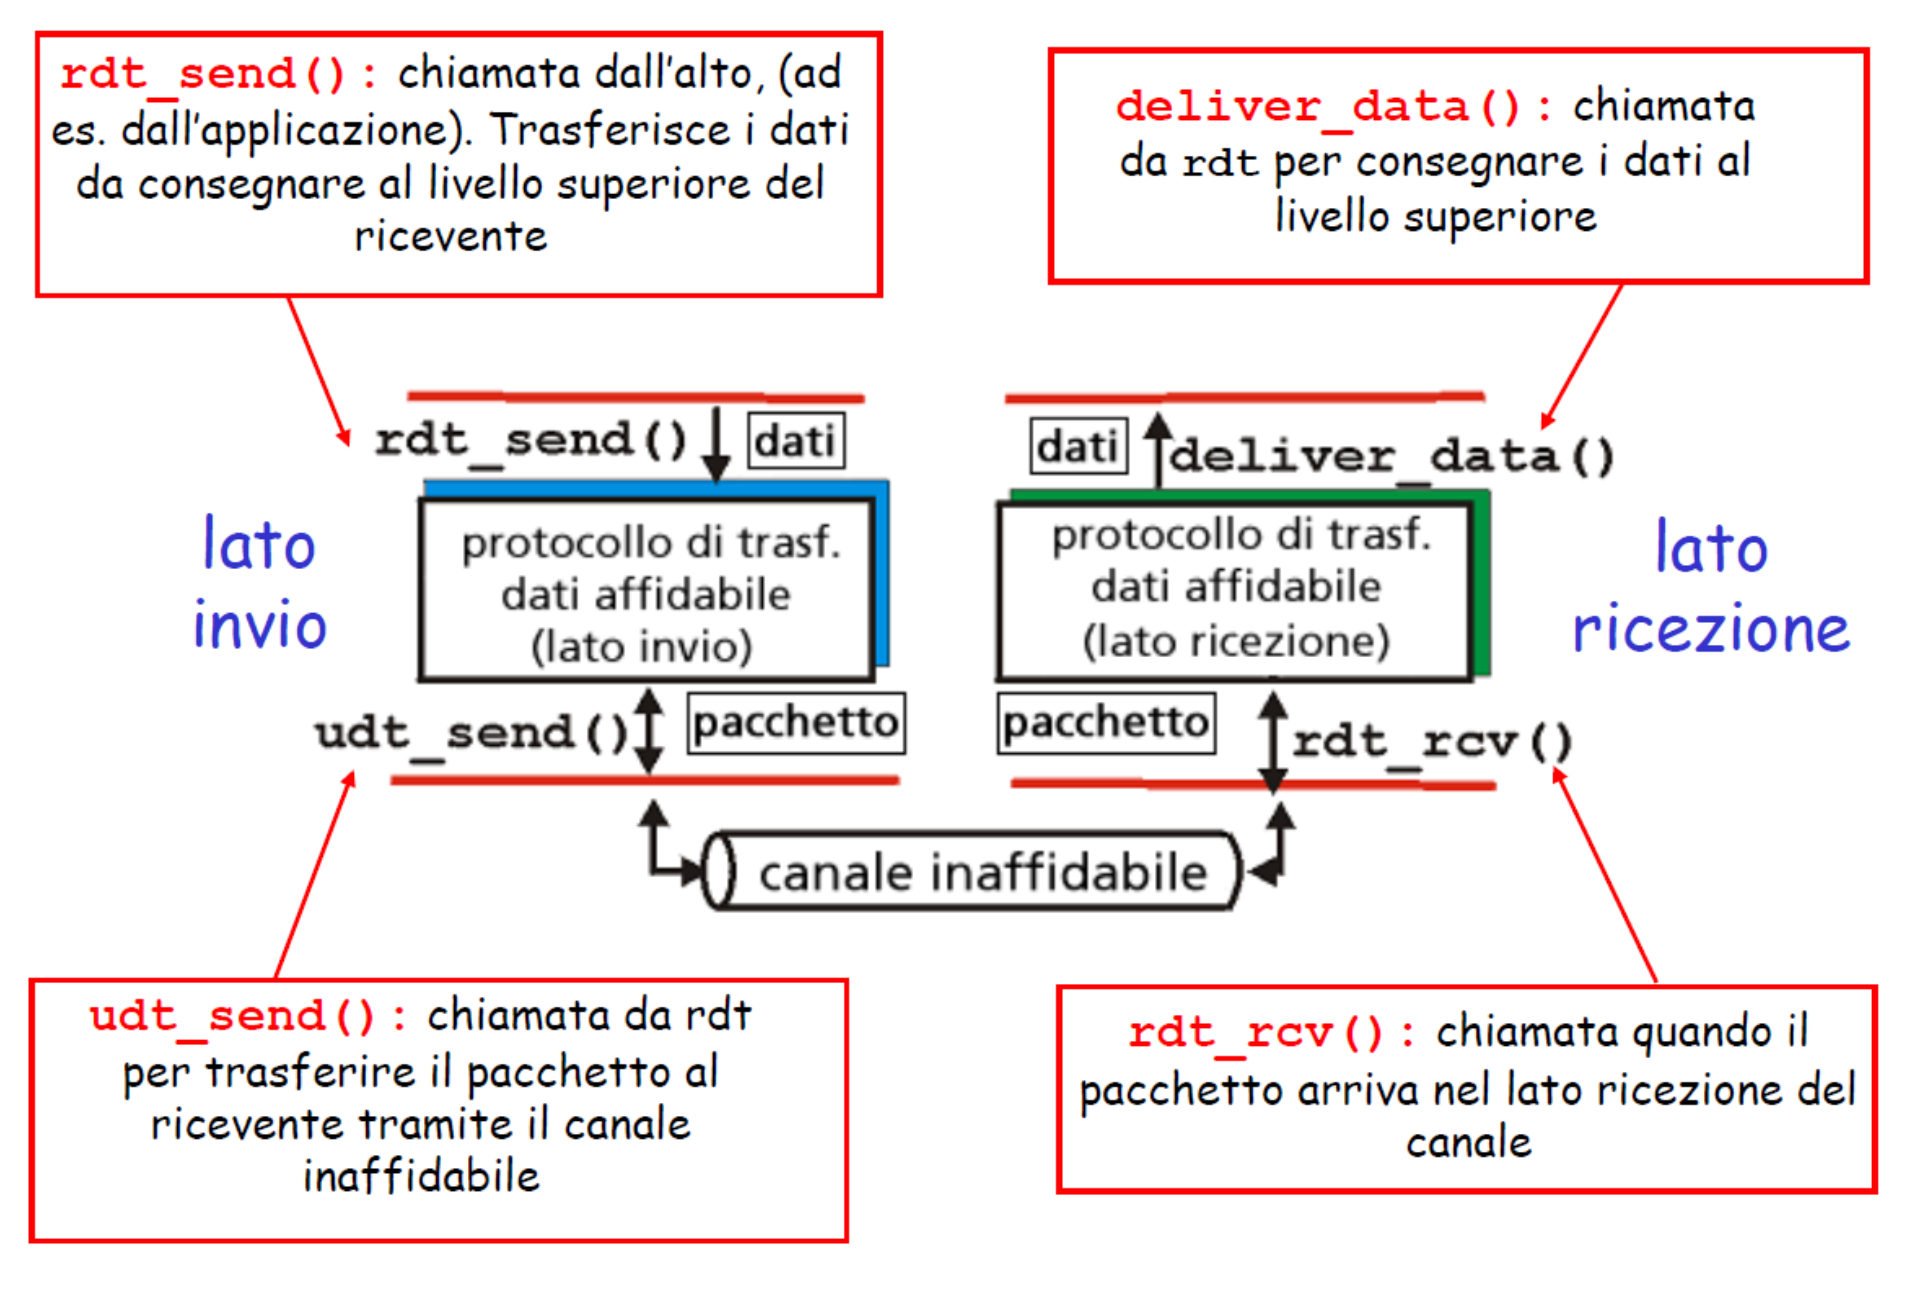
\includegraphics[width=0.7\linewidth]{rdt-1}
	\end{center}
	\paragraph{Stato di Rdt} Lo stato successivo a quello corrente è determinato unicamente dall'evento successivo
	\begin{center}
		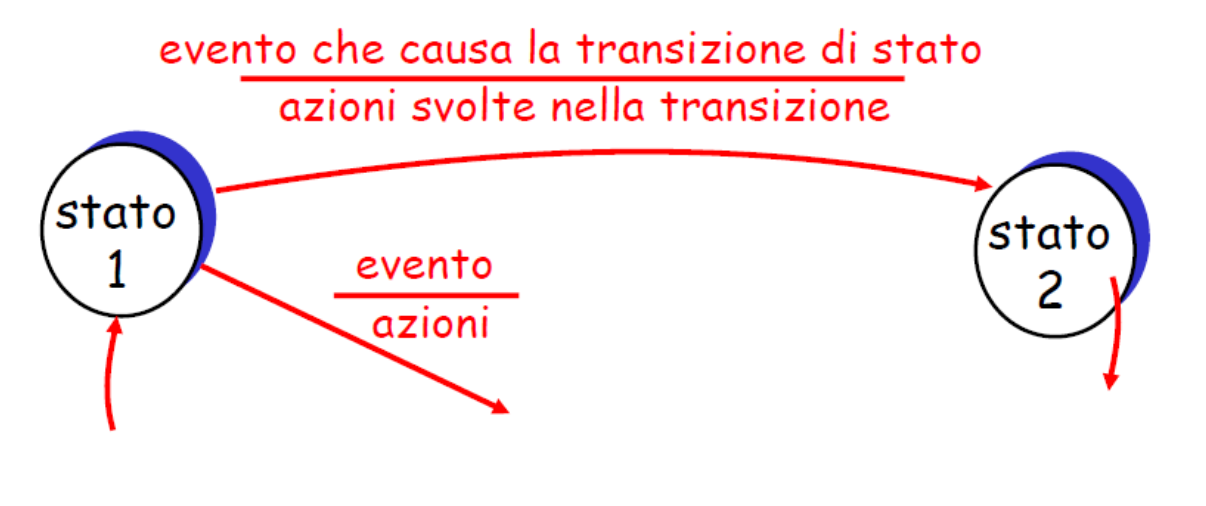
\includegraphics[width=0.7\linewidth]{rdt-stato}
	\end{center}
	\subsection{Rdt 1.0: trasferimento affidabile su canale affidabile}
	Il canale sottostante è perfettamente affidabile e è presente un automa distinto per mittente e ricevente.
	\subsection{Rdt 2.0: canale con errori nei bit}
	Il canale sottostante potrebbe confondere i bit nei pacchetti, si utilizza quindi il checksum per rilevare gli errori. Una volta ricevuto, con la notifica positiva \textbf{ACK} il ricevente comunica espressamente al mittente che il pacchetto ricevuto è corretto mentre con la notifica negativa \textbf{NAK} comunica che il pacchetto contiene errori. Se il mittente riceve un NAK verrà ritrasmesso il pacchetto.
	\medskip\\Con Rdt 2.0 sono stati introdotti nuovi meccanismi tra cui il rilevamento di errore e il feedback del destinatario (ACK e NAK).
	\medskip\\ Rdt 2.0 però ha un difetto fatale: se i pacchetti NAK e ACK sono danneggiati il mittente non saprà cos'è successo; non basta però ritrasmettere la notifica perché sono possibili duplicati.
	Il mittente ritrasmette quindi il pacchetto aggiungendo un numero di sequenza, e il ricevente lo scarterà se duplicato. Una volta inviato, il mittente aspetta la risposta del destinatario (\textit{stop and wait}).
	\subsection{Rdt 2.1}
	Il mittente aggiunge un numero di sequenza al pacchetto, saranno sufficienti due numeri (0 e 1). Dovrà poi controllare se gli ACK/NAK sono danneggiati e ricordarsi se il pacchetto corrente ha numero di sequenza 0 o 1.
	\medskip\\Il ricevente deve invece controllare se il pacchetto ricevuto è duplicato, lo stato indicherà se il numero di sequenza atteso è 0 o 1. Il ricevente non potrà però sapere se il suo ultimo ACK/NAK è stato ricevuto correttamente dal mittente.
	\subsection{Rdt 2.2: un protocollo senza NAK}
	Ha le stesse funzionalità di Rdt 2.1, utilizzando solamente gli ACK. In sostituzione al NAK il destinatario invierà un ACK per l'ultimo pacchetto ricevuto correttamente, il destinatario invece deve includere esplicitamente il numero di sequenza con l'ACK. Un ACK duplicato presso il mittente determina la stessa azione del NAK, cioè ritrasmettere il pacchetto corrente.
	 \subsection{Rdt 3.0: canali con errori e perdite}
	 Può succedere che il canale sottostante smarrisca i pacchetti (dati o ACK). Per ovviare a ciò il mittente attende un ACK per un tempo ragionevole, dopodiché, se non ricevuto, ritrasmetterà il pacchetto.
	 \medskip\\Se il pacchetto (o l'ACK) è solo in ritardo la trasmissione sarà duplicata, ma il problema è già gestita dai numeri di sequenza, che il destinatario specificherà anche nei pacchetti da riscontrare; è necessaria l'introduzione di un contatore.
	\begin{center}
		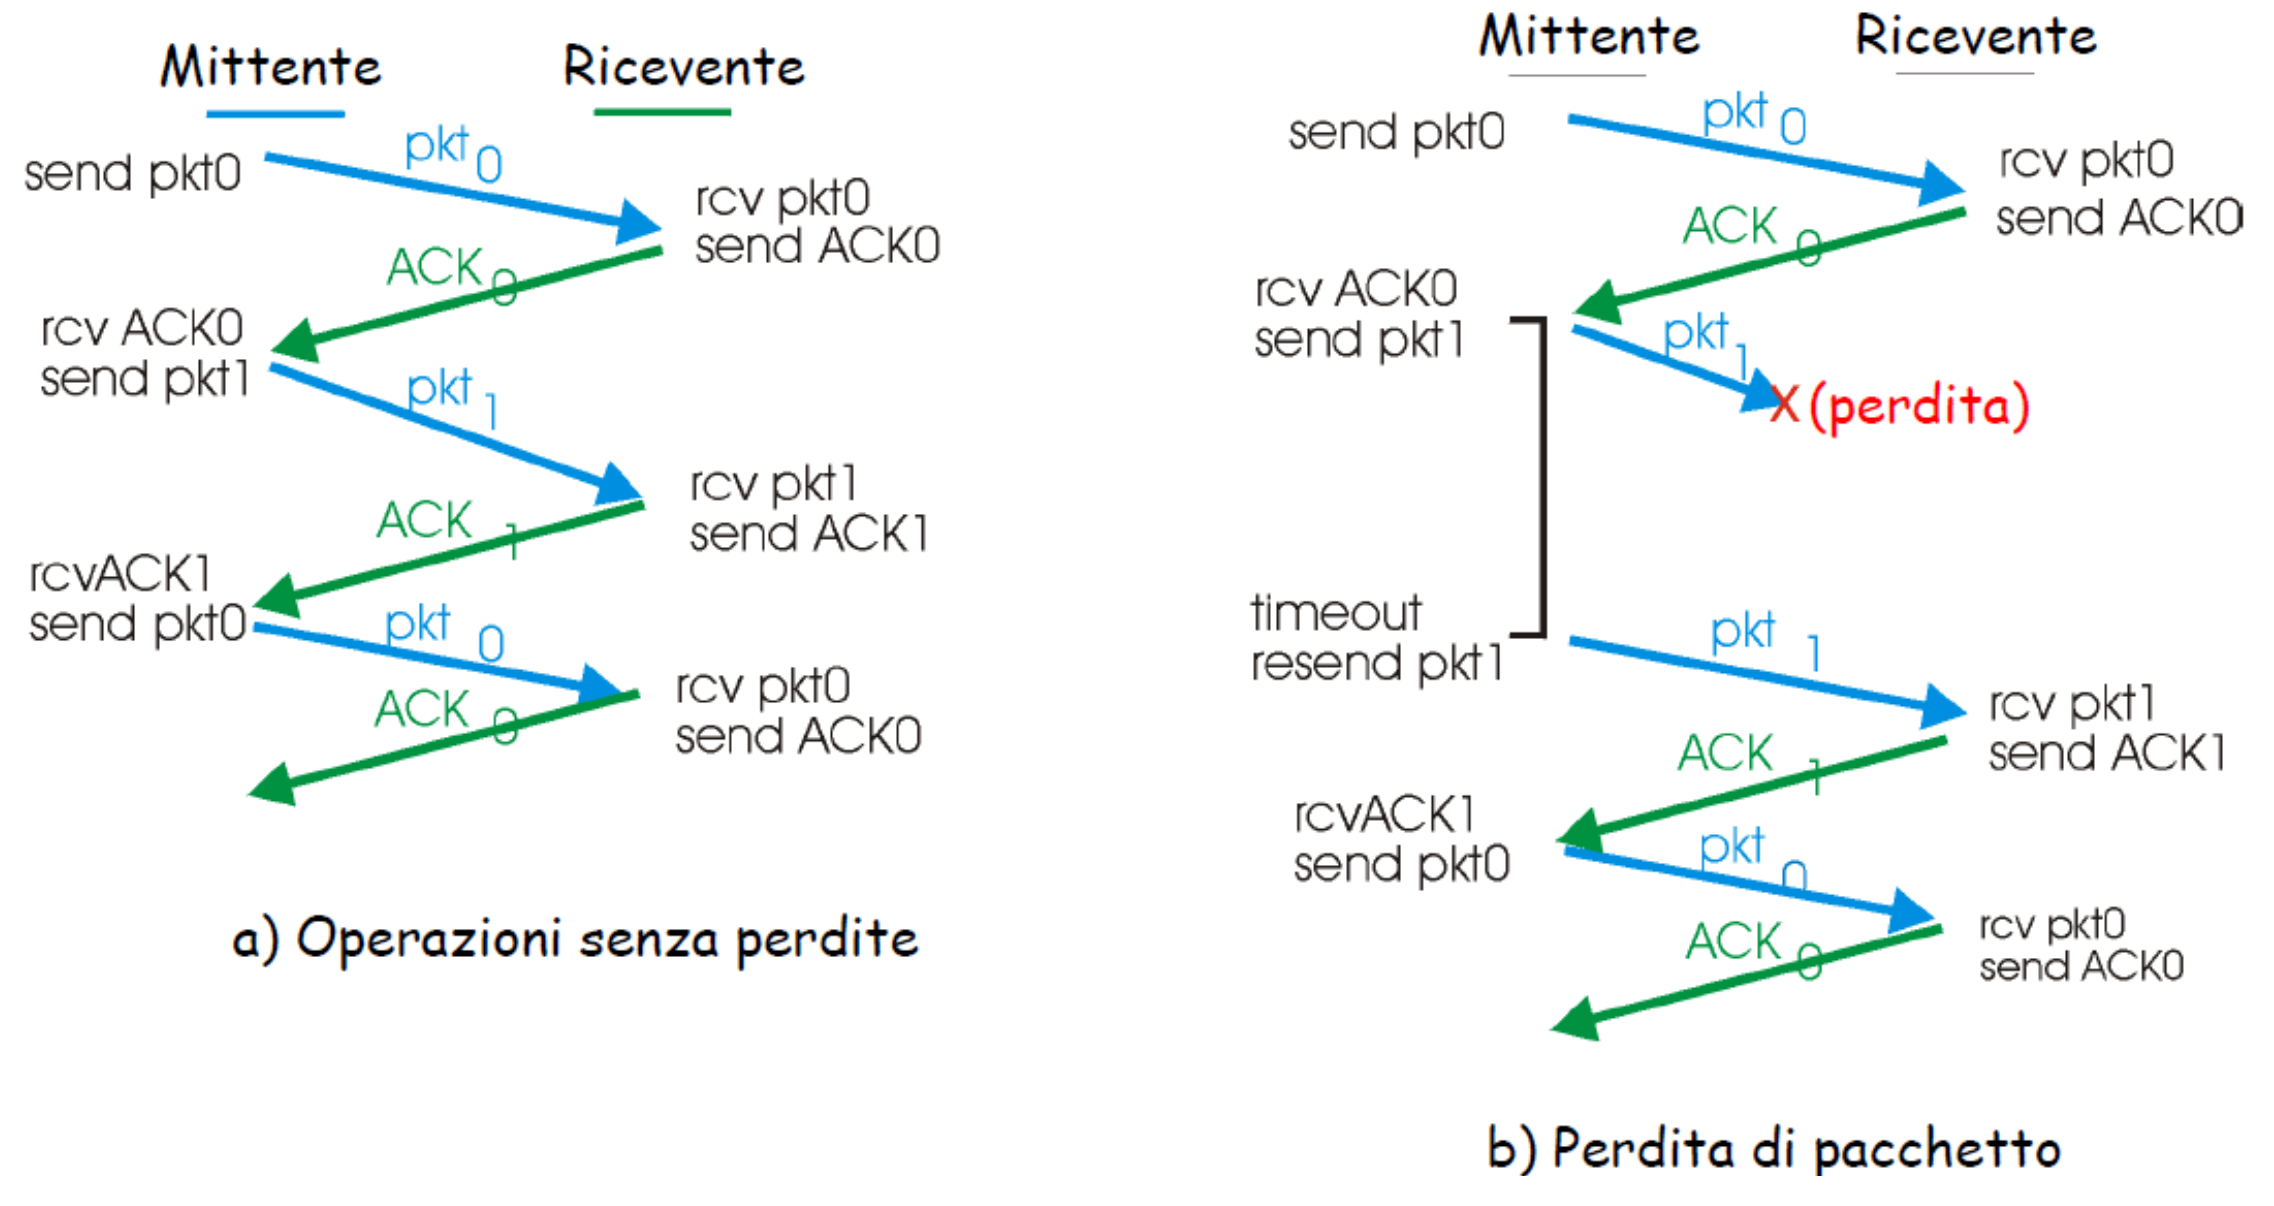
\includegraphics[width=0.7\linewidth]{rdt-2}
		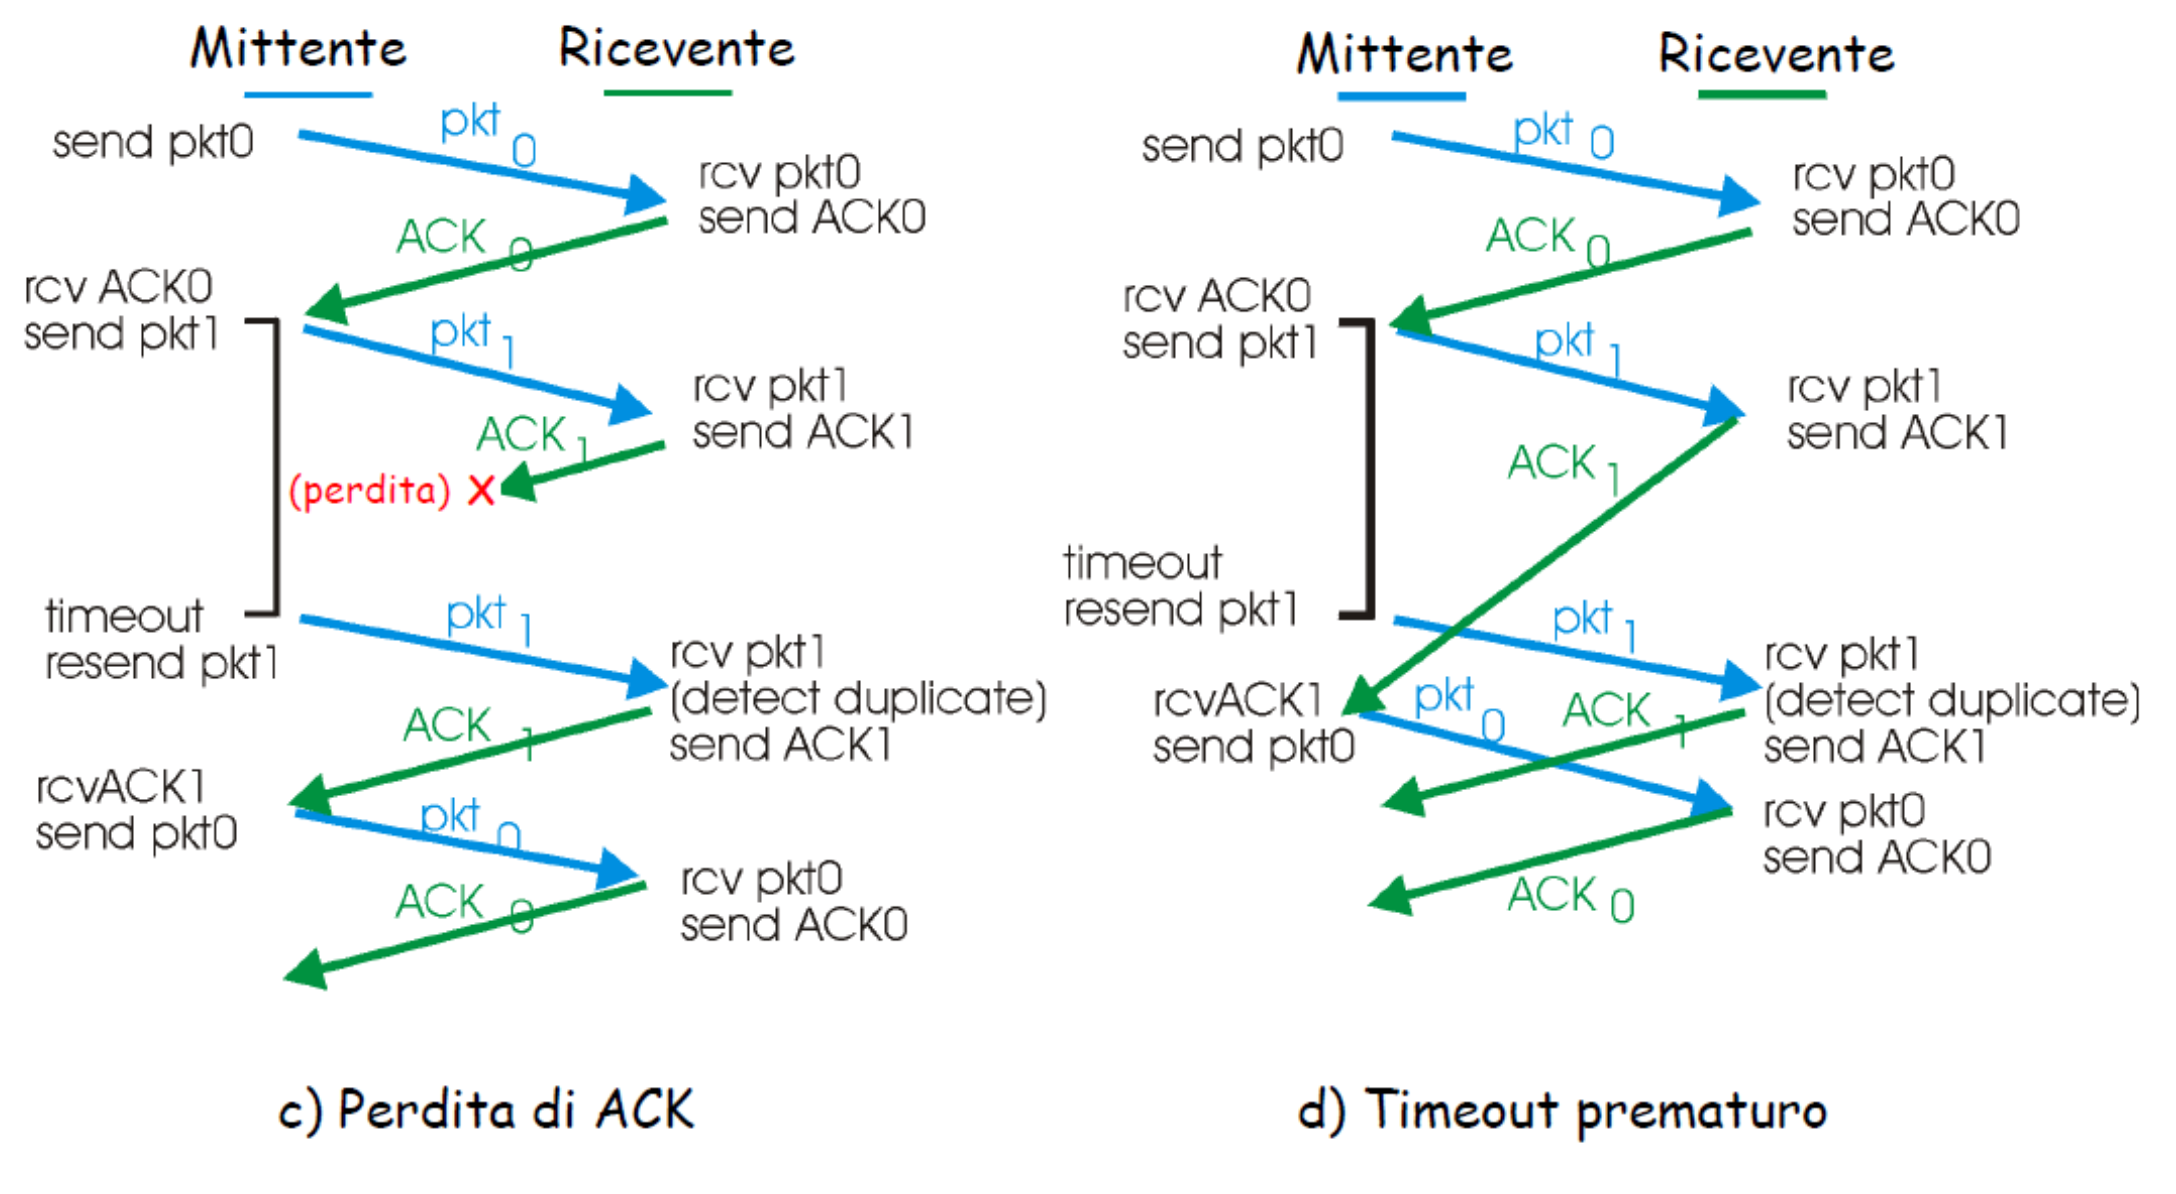
\includegraphics[width=0.7\linewidth]{rdt-3}
	\end{center}
	\subsection{Pipelining} Il mittente ammette più pacchetti in transito ancora da notificare, il loro numero di sequenza deve essere incrementale ed è presente un buffering dei pacchetti presso il mittente e il ricevente. Ci sono due forme generiche di protocolli con pipeline: \textit{Go-Back-N} e \textit{Ripetizione selettiva}.
	\subsubsection{Go-Back-N}
	\begin{itemize}
		\item Il mittente può avere fino a N pacchetti senza ACK in pipeline
		\item Il ricevente invia solo ACK cumulativi, non dà quindi l'ACK di un pacchetto se c'è un gap
		\item Il mittente ha un timer per il pacchetto più vecchio senza ACK.
	\end{itemize}
	\subsubsection{Ripetizione selettiva}
	\begin{itemize}
		\item Il mittente può avere fino a N pacchetti senza ACK in pipeline
		\item Il ricevente trasmette gli ACK solo sui singoli pacchetti.
		\item Il mittente mantiene un timer per ciascun pacchetto che non ha ancora ricevuto un ACK, che alla scadenza farà ritrasmettere solo i pacchetti senza ACK.
		\item Il ricevente accusa la ricevuta di ciascun singolo pacchetto.
	\end{itemize}
	\section{Trasporto orientato alla connessione: TCP}
	\begin{itemize}
		\item Implementa l'\textbf{Rdt 3.0} con pipelining
		\item \textbf{Connessione punto-punto}: un mittente e un destinatario
		\item Il flusso di byte è \textbf{affidabile} e in sequenza
		\item Il \textbf{controllo di flusso e di congestione} del TCP definiscono la dimensione della finestra di \textbf{pipelining}
		\item \textbf{Full-Duplex:} il flusso dei dati è bidirezionale nella stessa connessione e viene definita la dimensione massima del segmento (\textit{MSS})
		\item \textbf{Orientato alla connessione:} l'handshaking inizializza lo stato di mittente e destinatario prima di scambiare i dati
		\item \textbf{Flusso controllato:} il mittente non sovraccarica il destinatario
	\end{itemize}
	\begin{center}
		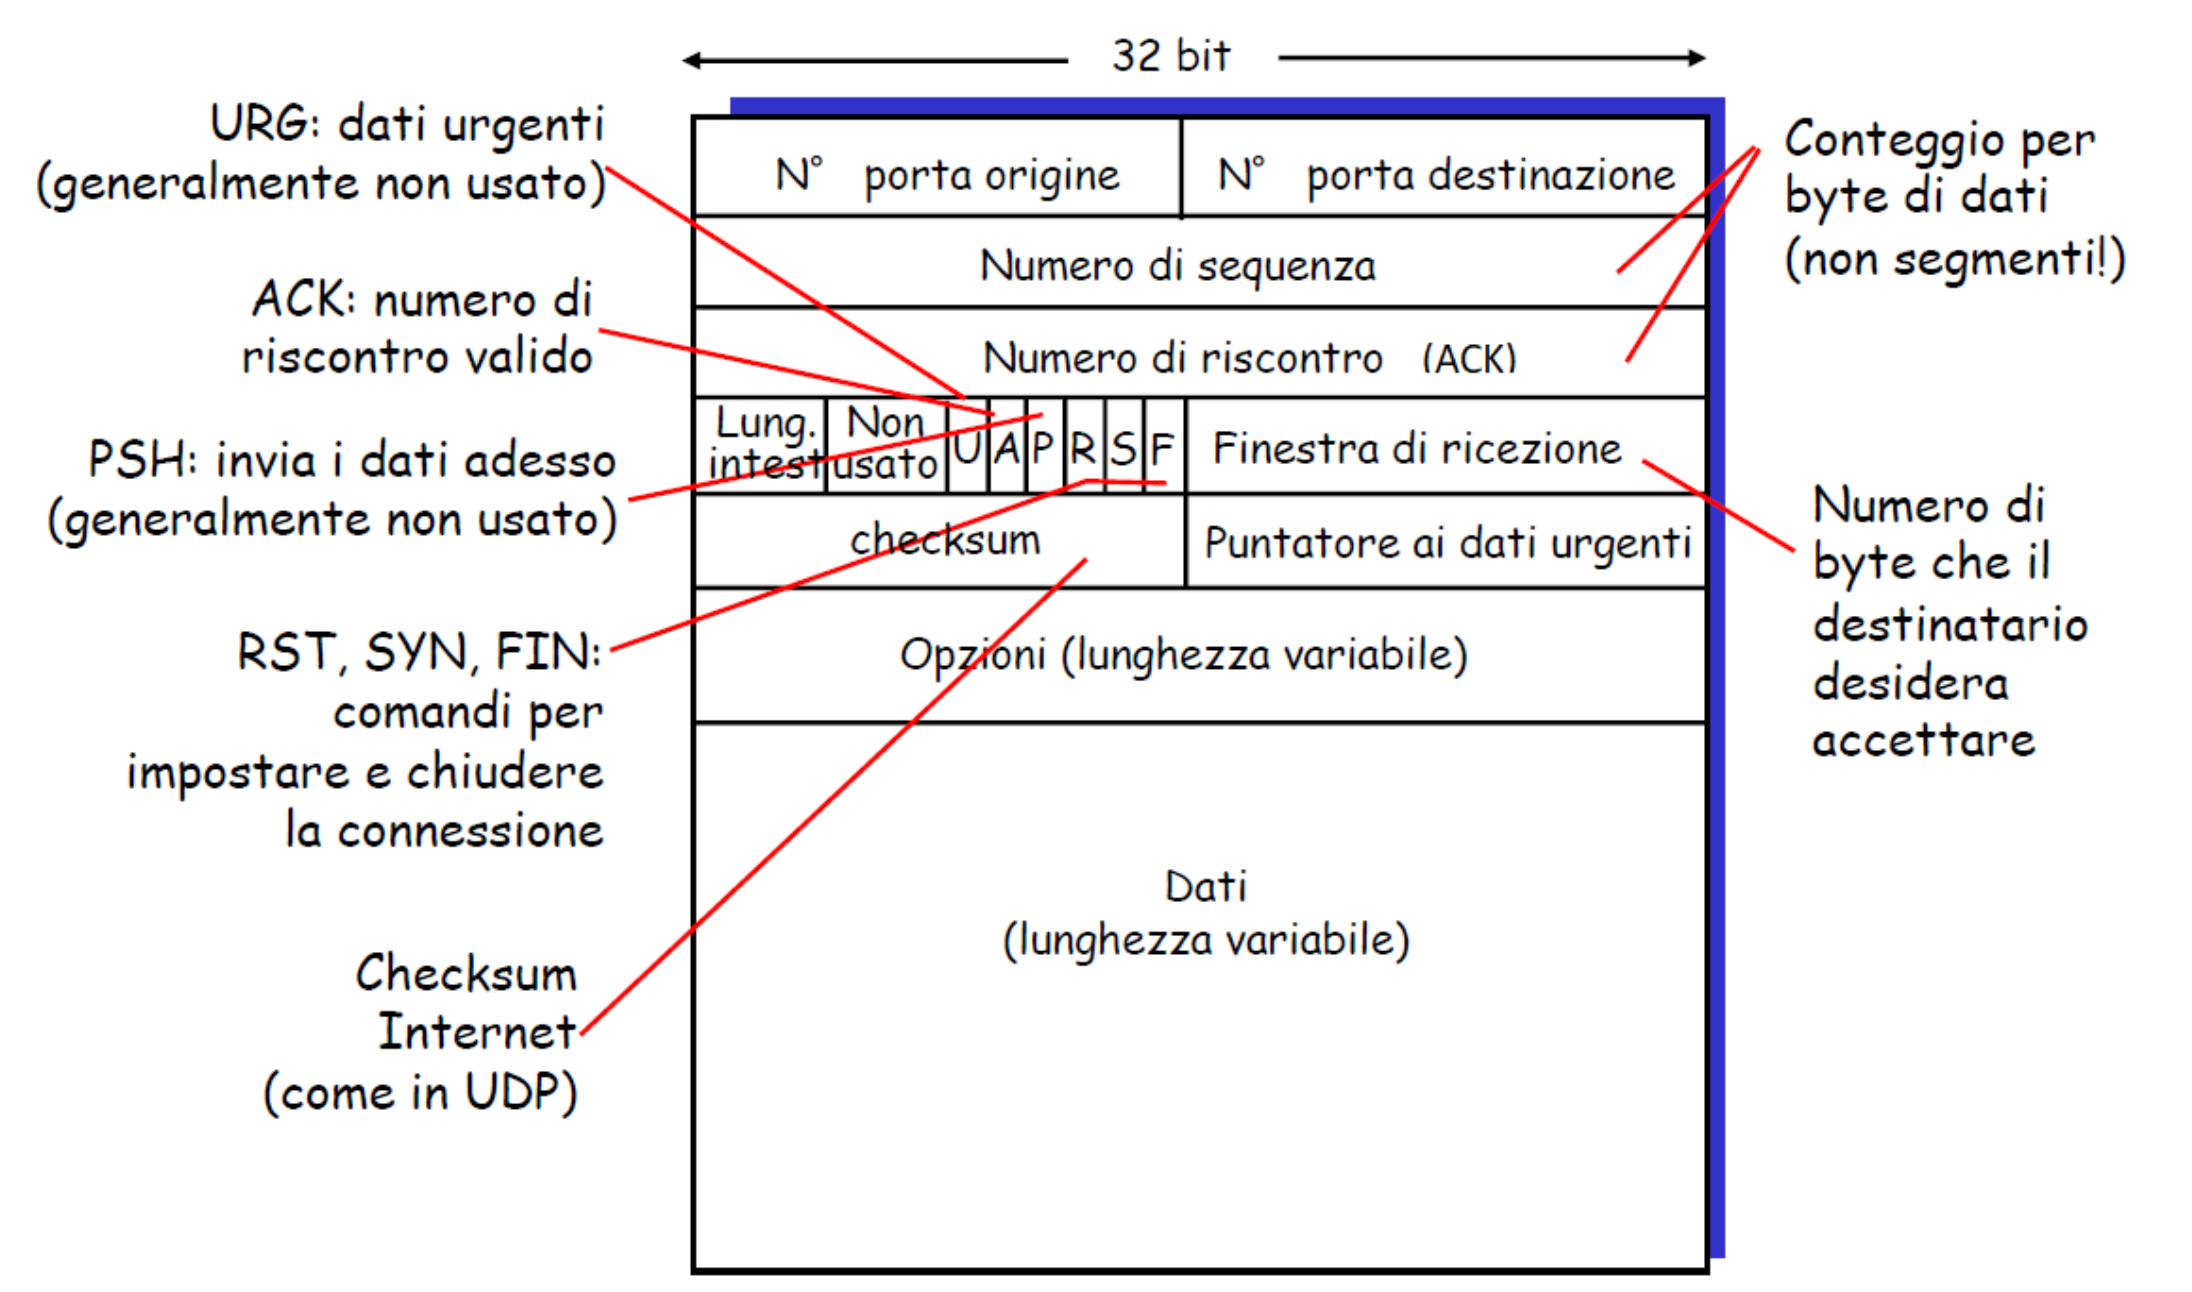
\includegraphics[width=0.7\linewidth]{segmento-tcp}
	\end{center}
	Alcuni dettagli sul segmento TCP:
	\begin{itemize}
		\item \textbf{Lunghezza dell'intestazione:} serve per sapere se ci sono informazioni nella parte opzionale, in caso negativo sarà di default 20 (5 righe \(\cdot\) 4 byte = 20)
		\item \textbf{Numero di sequenza:} numero del primo byte del segmento nel flusso di byte
		\item \textbf{ACK:} numero di sequenza del prossimo byte atteso
		\item Per calcolare il \textbf{timeout} si usa una media esponenziale ponderata
	\end{itemize}
	Il trasporto TCP crea un servizio di trasferimento dati affidabile sul servizio inaffidabile di IP. Le ritrasmissioni sono avviate da eventi di timeout e ACK duplicati.
	\begin{center}
		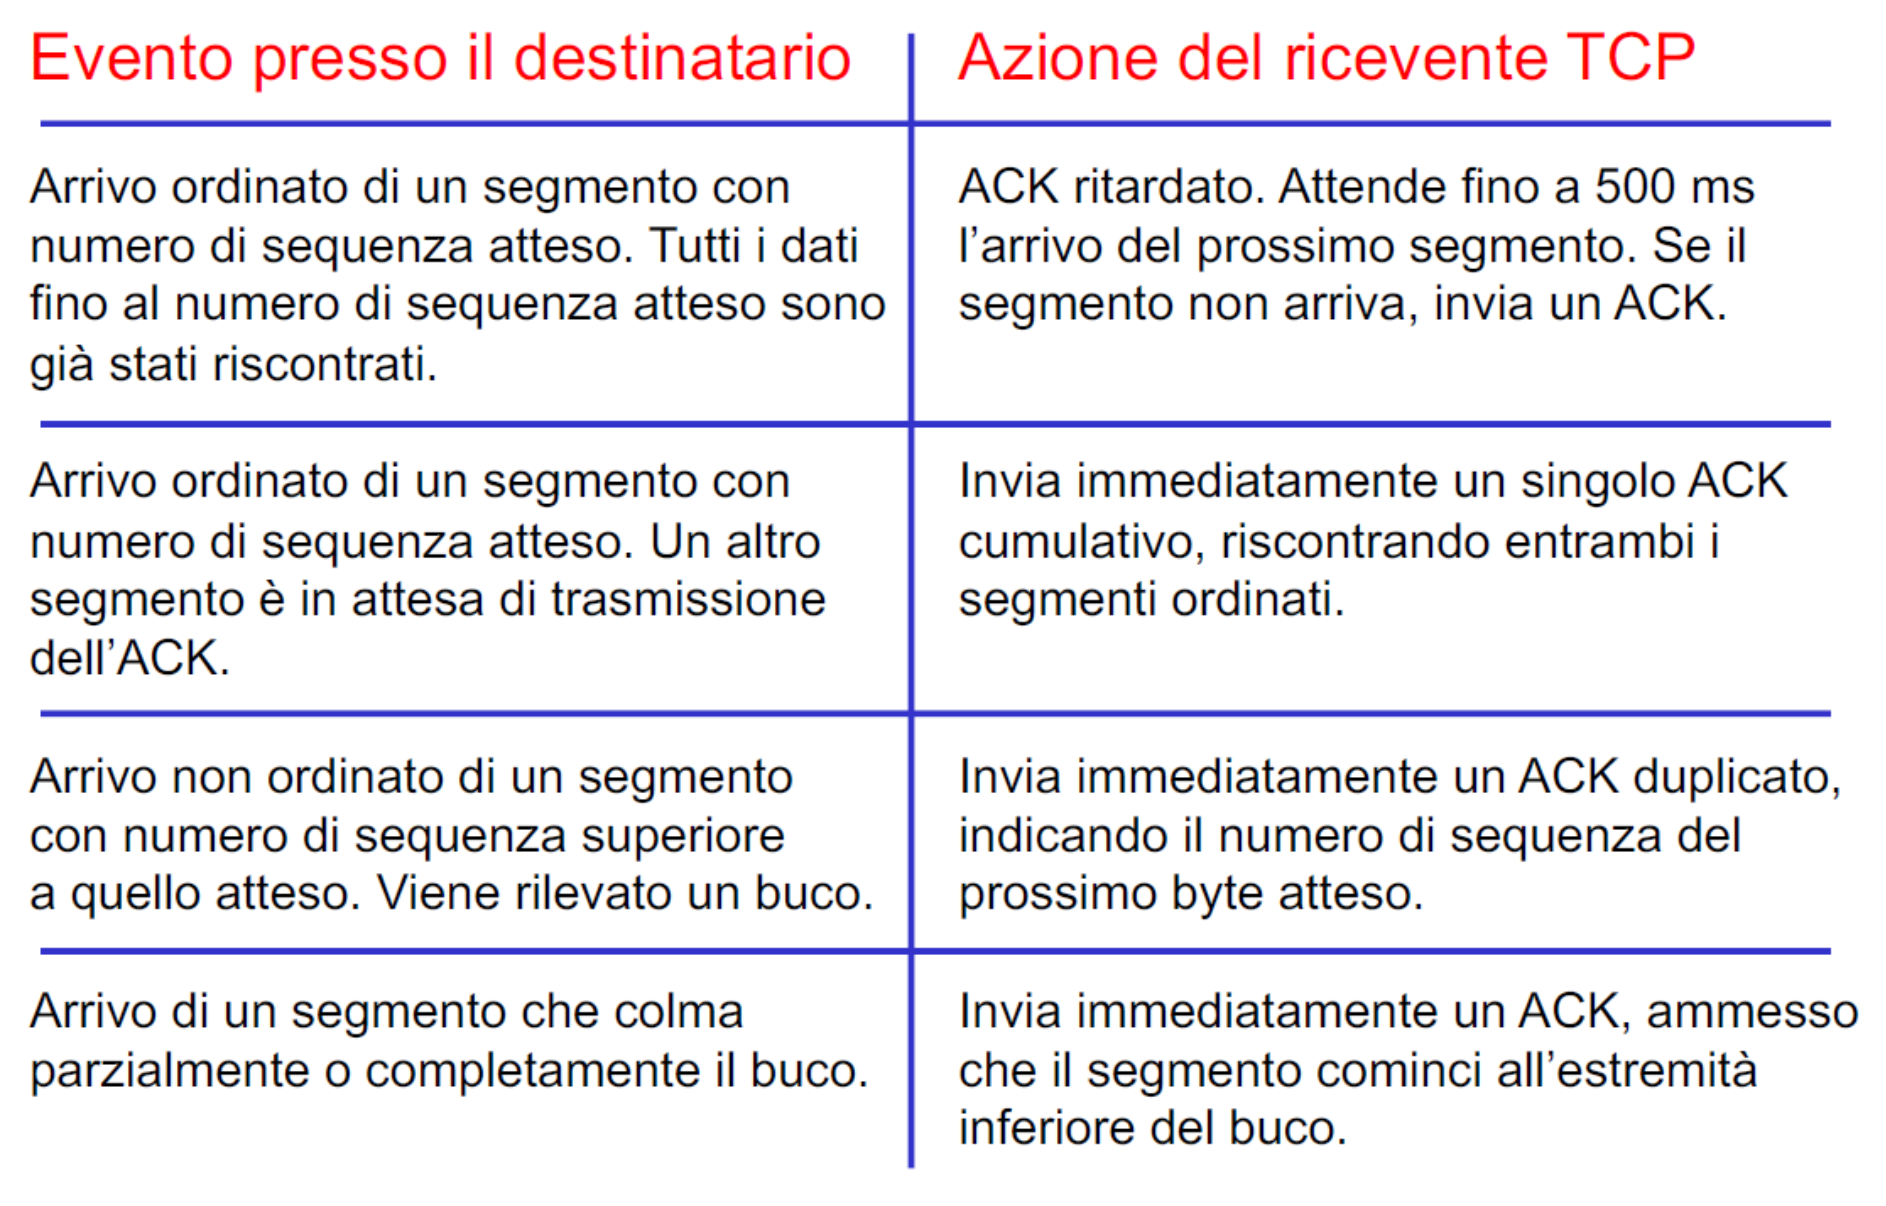
\includegraphics[width=0.7\linewidth]{eventi-tcp}
	\end{center}
	Il timeout spesso è relativamente lungo, si ha quindi un lungo ritardo prima che venga ritrasmesso il pacchetto perduto.
	\medskip\\Gli ACK perduti vengono rilevati tramite gli ACK duplicati: il mittente spesso invia molti segmenti, se un segmento viene smarrito è probabile che ci saranno molti ACK duplicati. Se il mittente riceve 3 ACK duplicati per lo stesso dato si suppone che il segmento che segue il dato riscontrato è andato perduto e rispedirà quindi il pacchetto prima che scada il timer (metodo di \textbf{trasmissione rapida}. 
	\subsection{TCP: controllo di flusso}
	\begin{wrapfigure}{r}{0.4\textwidth}
		\centering
		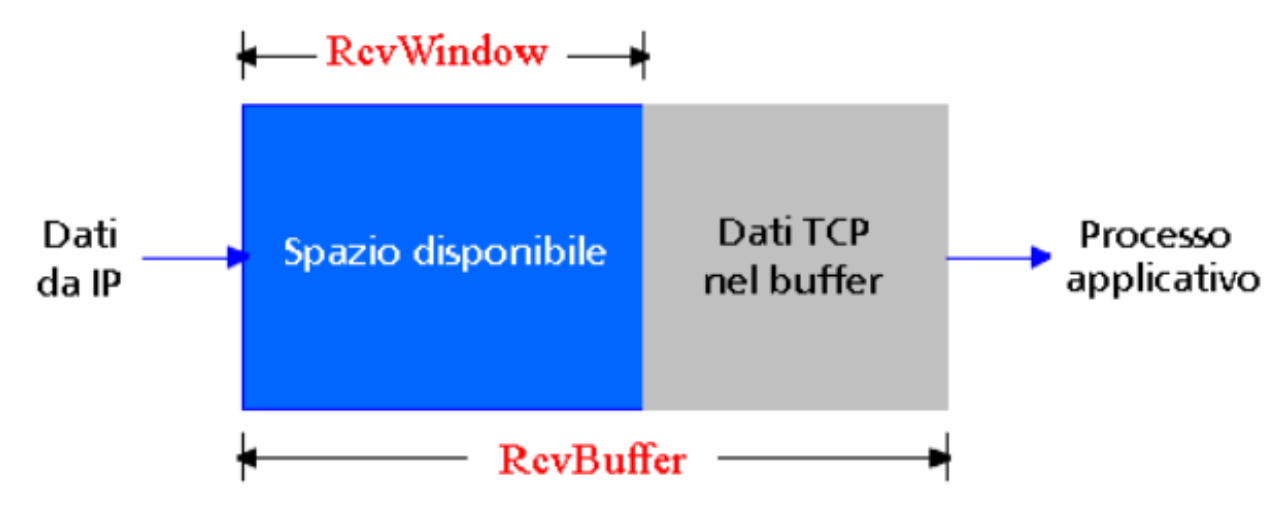
\includegraphics[width=0.4\textwidth]{controllo-di-flusso}
		\vspace{-20pt}
	\end{wrapfigure}
	
	Il lato ricevente della connessione TCP ha un buffer di ricezione, quindi il processo applicativo potrebbe essere rallentato dalla lettura del buffer. Con il controllo di flusso il mittente non vuole sovraccaricare il buffer del destinatario, trasmettendo troppi dati troppo velocemente. Il servizio di corrispondenza delle velocità indica che la frequenza di invio deve corrispondere alla frequenza di lettura dell'applicazione ricevente.
	\medskip\\Il destinatario comunica lo spazio disponibile includendo il valore \verb|RcvWindow| nei segmenti, il mittente limita i dati non riscontrati a \verb|RcvWindow| e garantisce che il buffer di ricezione non vada in overflow.
	
	\subsection{Gestione della connessione}
	La connessione viene gestita mediante un Handshake a tre vie:
	\begin{enumerate}
		\item Il client invia un segmento SYN al server che specifica il numero di sequenza iniziale, non viene inviato nessun dato
		\item Il server riceve il SYN e risponde con un segmento SYNACK e successivamente alloca i buffer
		\item Il client riceve SYNACK e risponde con un ACK che può anche contenere dati
	\end{enumerate}
	Per chiudere una connessione:
	\begin{enumerate}
		\item Il client invia un segmento di controllo FIN al server
		\item Il server riceve il segmento FIN e risponde con un ACK, chiude la connessione e invia un FIN
		\item Il client riceve il FIN e risponde con un ACK
		\item Il server riceve l'ACK e chiude la connessione
	\end{enumerate}
	
	\section{Principi del controllo di congestione}
	Per congestione si intende quando troppe sorgenti trasmettono troppi dati a una velocità talmente elevata che la rete non è in grado di gestirli. I sintomi della congestione possono essere pacchetti smarriti (causati da overflow nei buffer dei router) o lunghi ritardi (accodamento nei buffer).
	\medskip\\I due principali approcci al controllo di congestione sono:
	\begin{itemize}
		\item \textbf{Controllo di congestione punto-punto}
		\begin{itemize}
			\item Nessun supporto esplicito dalla rete
			\item La congestione è dedotta osservando le perdite e i ritardi nei sistemi terminali
			\item Metodo adottato da TCP
		\end{itemize}
		\item \textbf{Controllo di congestione assistito dalla rete}
		\begin{itemize}
			\item I router forniscono un feedback ai sistemi terminali
			\item Utilizzato un singolo bit per indicare la congestione
			\item Viene comunicata in modo esplicito al mittente la frequenza trasmissiva
		\end{itemize}
	\end{itemize}
	\section{Controllo di congestione in TCP (AIMD)}
	Il controllo di congestione in TCP viene effettuato mediante l'approccio AIMD; ovvero incremento additivo e decremento moltiplicativo.
	\medskip\\Consiste nell'aumentare il tasso trasmissivo sondando la rete fino a quando non si verifica una perdita. Secondo l'\textbf{incremento adattivo} fa aumentare la \verb|CongWin| di 1 MSS a ogni RTT in assenza di perdita, mentre secondo il \textbf{decremento moltiplicativo} riduce a metà \verb|CongWin| dopo un evento di perdita. La formula diventa quindi approssimativamente:
	\begin{displaymath}
  		\text{Frequenza d'invio = }\frac{CongWin}{RTT}\text{ byte/sec}
	\end{displaymath}
	
	\verb|CongWin| è una funzione dinamica della congestione percepita. Il mittente percepisce la congestione dopo un evento di perdita, quindi un timeout o una ricezione di 3 ACK duplicati, e riduce di conseguenza la frequenza di invio (\verb|CongWin|).
	\medskip\\Vengono utilizzati tre meccanismi: AIMD, partenza lenta e reazione agli eventi di timeout.
	\newpage
	\subsection{Partenza lenta}
	\begin{wrapfigure}{r}{0.3\textwidth}
		\centering
		\vspace{-20pt}
		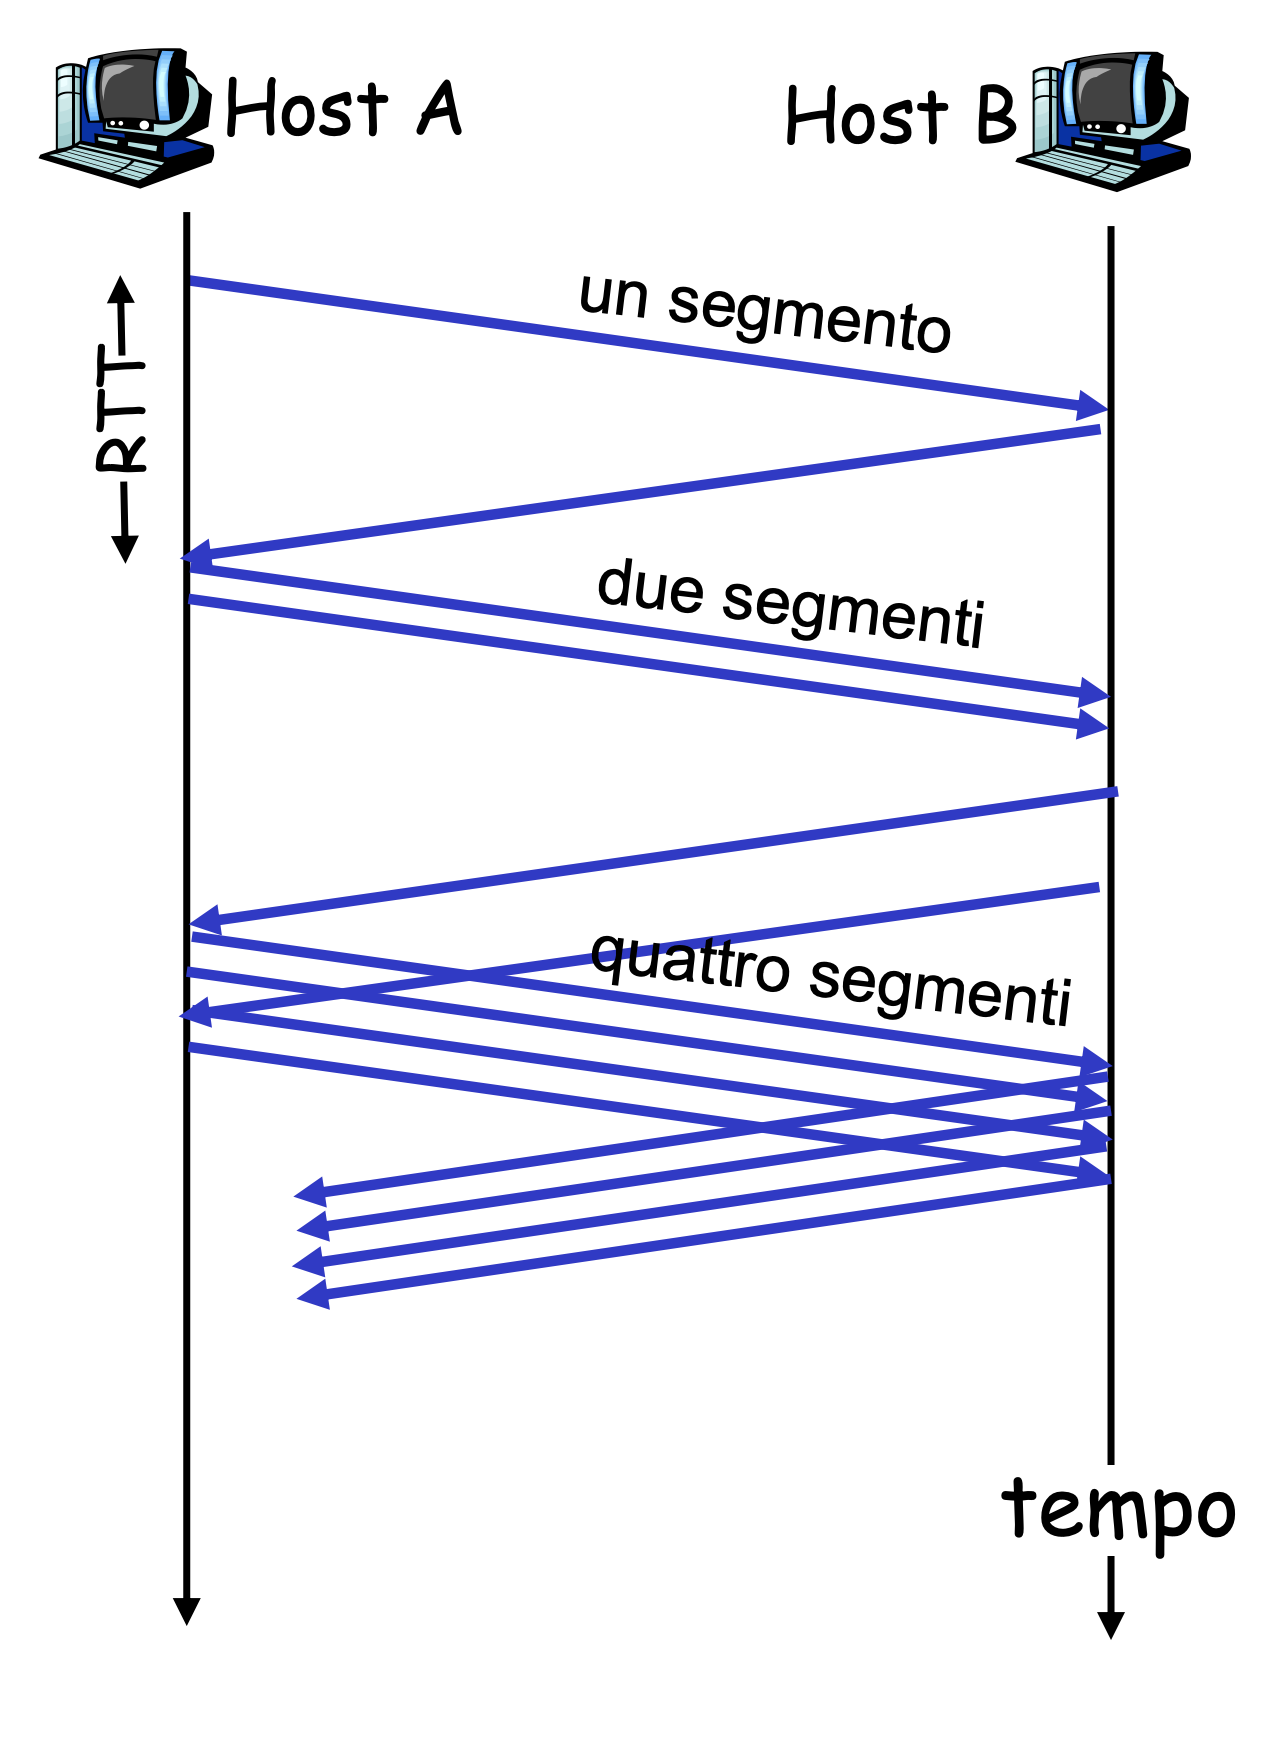
\includegraphics[width=0.3\textwidth]{partenza-lenta}
		\vspace{-50pt}
	\end{wrapfigure}
	Quando si stabilisce una connessione (\verb|CongWin| = 1 MSS) la frequenza aumenta in modo esponenziale fino a quando non si verifica una perdita: infatti \verb|CongWin| raddoppia a ogni RTT incrementandolo per ogni ACK ricevuto.
	\medskip\\Dopo 3 ACK duplicati (perdita), \verb|CongWin| è ridotto a metà e la finestra cresce linearmente. Se si verifica però un timeout, \verb|CongWin| viene impostato a 1 MSS crescendo in modo esponenziale fino a una soglia, dopo la quale crescerà linearmente.
	\medskip\\La filosofia seguita è quella che 3 ACK duplicati indicano la capacità della rete di consegnare qualche segmento, mentre un timeout prima di 3 ACK duplicati è "più allarmante".
	\medskip\\La soglia impostata è variabile, ma in caso di perdita la soglia diventa \(\frac{1}{2}\) di \verb|CongWin| appena prima dell'evento.
	\subsection{Riassunto: controllo di congestione}
	\begin{itemize}
		\item Quando \verb|CongWin| è sotto la soglia, il mittente è nella fase di \textbf{partenza lenta}; la finestra cresce in modo esponenziale.
		\item Quando \verb|CongWin| è sopra la soglia, il mittente p nella fase di \textbf{congestion avoidance}; la finestra cresce in modo lineare.
		\item Quando si verificano \textbf{tre ACK duplicati}, il valore della soglia viene impostato a \verb|CongWin/2| e \verb|CongWin| viene impostata al valore della soglia.
		\item Quando si verifica un \textbf{timeout}, il valore della soglia viene impostato a \verb|CongWin/2| e \verb|CongWin| è impostata a 1 MSS.
	\end{itemize}
	\subsection{Throughput TCP}
	Il throughput medio di TCP varia in funzione della dimensione della finestra e di RTT. Se, dopo una perdita, la finestra è W, il throughput sarà W/RTT. Dopo la perdita la finestra diventerà W/2 e il throughput di conseguenza diventa W/2RTT. Il throughput medio è quindi 0.75 W/RTT
	\subsection{Equità di TCP}
	\paragraph{Equità} se K sessioni TCP condividono lo stesso collegamento con ampiezza di banda R (collo di bottiglia), ogni sessione dovrà avere una frequenza trasmissiva media pari a R/K.
	\medskip\\TCP infatti è equo perché con due connessioni in concorrenza l'incremento additivo ha una pendenza pari a 1, mentre il decremento moltiplicativo riduce il throughput in modo proporzionale.
	\medskip\\Proprio per questo le applicazioni multimediali spesso usano UDP, poiché non vogliono che il loro tasso trasmissivo venga ridotto ma tollerano la perdita di pacchetti.
	\chapter{Il livello di collegamento}
	
	
	
	
\end{document}